\documentclass[journal,10pt]{IEEEtran}
\usepackage[brazil]{babel}
\usepackage{lmodern}
\usepackage{amsmath,amssymb}
\usepackage{graphicx}
\usepackage{booktabs}
\usepackage{url}
\usepackage[hidelinks]{hyperref}
\graphicspath{{fig/}}

\title{Imagem a\'erea estereosc\'opica a partir de um \'unico telefone e de uma fatia do espelho ``Mirage'':\\ um estudo sistem\'atico por tra\c{c}ado de raios}

\author{Anderson~Alves~dos~Santos%
\thanks{A.~A.~dos Santos \'e acad\^emico do curso de Intelig\^encia Artificial e Machine Learning (IAM), turma FLD6662753CET, da Universidade Leonardo da Vinci. Trabalho desenvolvido para a disciplina Intelig\^encia Artificial Simb\'olica (234976) no \^ambito do projeto Holosion.}%
\thanks{Manuscrito preparado em novembro de 2026 a partir dos simuladores e do registro de medidas do projeto Holosion. Todos os valores num\'ericos foram obtidos por tra\c{c}ado de raios vetorial sobre superf\'icies anal\'iticas; nenhum dispositivo f\'isico foi constru\'ido at\'e a data deste texto.}}

\markboth{Santos --- Holosion: imagem a\'erea por tra\c{c}ado de raios}{}

\begin{document}
\maketitle

\begin{abstract}
O brinquedo ``Mirage'' forma uma imagem real flutuante de um objeto deitado no leito de um par de espelhos parab\'olicos. Investigamos, por tra\c{c}ado de raios vetorial, se um \'unico telefone celular e um \'unico recorte desse espelho podem substituir o objeto, o motor e o segundo espelho e ainda produzir uma imagem a\'erea com profundidade. Partindo das t\'ecnicas que validamos no par completo (rotor de voxels, telas no lugar de cada espelho, p\'etalas no plano focal, presets elipsoidais), relatamos uma sequ\^encia de dezoito tentativas com um \'unico espelho, cada uma medida com a mesma r\'egua: converg\^encia de raios por m\'inimos quadrados, vista do olho tra\c{c}ada pixel a pixel, pupila de 4~mm, dois olhos separados de 64~mm e cabe\c{c}a em movimento. Os principais achados s\~ao: (i) com um \'unico espelho do tamanho do telefone, o olho nunca v\^e a tela inteira --- o espelho precisa estender-se por baixo da abertura (35/35 pontos vistos, janela de 220$\times$720~mm, caixa de 11,7~L); (ii) a imagem real de uma tela plana \'e uma l\^amina inclinada sem profundidade pr\'opria, e os dois olhos compartilham os mesmos pixels (erro de 4,6~mm por olho); (iii) a profundidade verdadeira exige o telefone no plano focal e uma abertura menor que a dist\^ancia interocular, o que separa os pixels por olho (0,1~\% de vazamento) e reconstr\'oi um cubo de 30~mm com erro m\'edio de 0,64~mm, ao custo de usar 15$\times$16~mm da tela e de um conflito verg\^encia--acomoda\c{c}\~ao de 2--4~D; (iv) a nitidez \'e governada pelo espelho (borr\~ao de $\approx$0,75~mm para $f=80{,}6$~mm, independente do tamanho do pixel), enquanto a precis\~ao de profundidade \'e governada pelo pixel (1,54~mm $\to$ 0,24~mm de 0,13 a 0,016~mm); (v) inclinar o espelho em 16$^\circ$ com o telefone acompanhando o foco n\~ao reduz o borr\~ao, mas baixa o \^angulo de observa\c{c}\~ao de 88,5$^\circ$ para 72,5$^\circ$. Tornamos toda a cadeia determin\'istica (gerador com semente, rel\'ogio congel\'avel), exportamos as geometrias finais em 3MF e desenvolvemos um jogo original em tempo real que \'e exibido exclusivamente atrav\'es dos raios tra\c{c}ados, em todas as configura\c{c}\~oes. Conclu\'imos que tela inteira, volume do conte\'udo e foco sem conflito n\~ao s\~ao simultaneamente ating\'iveis com um espelho e uma tela plana, e quantificamos cada compromisso.
\end{abstract}

\begin{IEEEkeywords}
imagem a\'erea, espelho parab\'olico, campo de luz, estereoscopia, tra\c{c}ado de raios, conflito verg\^encia--acomoda\c{c}\~ao, pr\'e-compensa\c{c}\~ao.
\end{IEEEkeywords}

\section{Introdu\c{c}\~ao}
Dois espelhos c\^oncavos parab\'olicos unidos pela borda, o superior com um furo central, formam acima do furo uma imagem real do que est\'a no leito do inferior. O efeito \'e vendido como brinquedo h\'a d\'ecadas~\cite{optigone} e discutido em ensino de \'optica~\cite{etop2015}: a imagem \'e real, flutua no ar e pode ser observada de uma coroa de dire\c{c}\~oes. N\~ao \'e um holograma --- n\~ao h\'a fase reconstru\'ida~\cite{bornwolf1999} --- mas uma imagem \'optica comum, com acomoda\c{c}\~ao correta e paralaxe cont\'inua, o que a torna mais confort\'avel do que a maioria dos mostradores autoestereosc\'opicos~\cite{dodgson2005,hoffman2008}.

O ponto de partida deste trabalho foi substituir o objeto f\'isico por uma fonte program\'avel. A pergunta evoluiu, por press\~ao de portabilidade, at\'e a forma mais econ\^omica imagin\'avel: um telefone celular, um \'unico recorte de espelho com a curvatura do Mirage e uma caixa preta. O que se perde e o que se ganha a cada simplifica\c{c}\~ao?

Respondemos com um programa de simula\c{c}\~ao em que \emph{nada da imagem \'e desenhado}: cada ponto vis\'ivel \'e a converg\^encia de raios tra\c{c}ados, e cada quadro ``visto pelo olho'' \'e obtido por tra\c{c}ado inverso pixel a pixel. A contribui\c{c}\~ao n\~ao \'e um dispositivo, mas um mapa quantitativo do espa\c{c}o de projeto, com os becos sem sa\'ida inclu\'idos.

\section{Fundamentos}
\subsection{O par parab\'olico e seu \'unico ponto perfeito}
Para dois paraboloides de mesma semi-abertura $R$ e flecha $s$, a focal de cada um \'e $f = R^2/4s$. Existe um \'unico arranjo sem aberra\c{c}\~ao, quando o foco de cada espelho cai no v\'ertice do outro: $s = R/2\sqrt{2}$ e separa\c{c}\~ao de v\'ertices $D = 2s = f$. Verificamos por tra\c{c}ado que nesse ponto o RMS axial \'e nulo dentro da precis\~ao num\'erica ($\sim10^{-14}$~mm), com aumento transversal $m_t = -1$ em ambos os eixos e longitudinal $m_L = +1$. O determinante $(-1,-1,+1)$ \'e positivo: a imagem \emph{n\~ao} \'e invertida nem espelhada, e sim o objeto girado 180$^\circ$ em torno do eixo vertical. Fora desse ponto a degrada\c{c}\~ao n\~ao \'e gradual: o feixe converge fora do plano do furo e a imagem desaparece em vez de borrar.

\subsection{Um \'unico espelho fora de eixo}
Removido o espelho superior, resta um espelho c\^oncavo usado fora de eixo com uma tela em $u$ do v\'ertice. Na aproxima\c{c}\~ao paraxial $1/u + 1/v = 1/f$ com $f = R_v/2$, sendo $R_v$ o raio de curvatura no v\'ertice ($z = r^2/2R_v$ para o paraboloide). Tr\^es regimes importam aqui: (a) $u > f$ forma imagem real, inclinada e curva, cujo aumento cresce quando $u \to f^{+}$; (b) $u = f$ transforma cada pixel em um feixe paralelo, isto \'e, em uma \emph{dire\c{c}\~ao}; (c) $u < f$ forma imagem virtual atr\'as do espelho. O regime (b) \'e o das ``p\'etalas'' da terceira aba do simulador principal e, como mostraremos, \'e o \'unico que separa os pixels por olho com uma \'unica tela.

\subsection{Invariante e or\c{c}amento de informa\c{c}\~ao}
O invariante de Lagrange~\cite{hecht2017} liga campo, abertura e resolu\c{c}\~ao: ampliar a imagem reduz o lobo de observa\c{c}\~ao e o n\'umero de pontos resolvidos na mesma propor\c{c}\~ao. A especifica\c{c}\~ao do projeto~\cite{holosion2026} registra esse pre\c{c}o para o par elipsoidal estigm\'atico ($D = 278$~mm): $\times1$ d\'a 81 pontos e lobo de 20$^\circ$; $\times3$ d\'a 24 pontos e lobo de 7$^\circ$. Nenhuma das tentativas abaixo escapa dessa conta.

\section{M\'etodo}
\subsection{N\'ucleo de tra\c{c}ado}
As superf\'icies s\~ao anal\'iticas (paraboloide, elipsoide prolato, esfera, planos); as interse\c{c}\~oes resolvem a quadr\'atica correspondente~\cite{spencer1962}, restritas ao recorte e, quando h\'a caixa, \`as paredes e \`a tampa que cortam o espelho. A reflex\~ao \'e $\mathbf d' = \mathbf d - 2(\mathbf d\cdot\hat{\mathbf n})\hat{\mathbf n}$. O ponto imagem de um pixel \'e a solu\c{c}\~ao de m\'inimos quadrados sobre as retas de sa\'ida, $\sum_i (I - \hat{\mathbf d}_i\hat{\mathbf d}_i^{\mathsf T})\,\mathbf X = \sum_i (I - \hat{\mathbf d}_i\hat{\mathbf d}_i^{\mathsf T})\,\mathbf X_i$, e n\~ao a interse\c{c}\~ao com um plano: isso captura a curvatura de campo sem hip\'otese pr\'evia. A pupila \'e amostrada por espiral de \^angulo \'aureo.

\subsection{O que o olho v\^e}
Cada pixel do quadro do observador \'e um raio lan\c{c}ado do olho, que atravessa a abertura (vidro fum\^e, 4~\% de brilho da sala), reflete no espelho e cai --- ou n\~ao --- em um pixel da tela; o corpo do telefone e as paredes bloqueiam. Para medir distor\c{c}\~ao, o ponto \emph{aparente} de um pixel para um olho \'e obtido por Newton sobre o ponto do espelho cujo reflexo atinge o olho, seguido de um feixe do tamanho da pupila; o RMS desse feixe \'e o borr\~ao.

\subsection{Pr\'e-compensa\c{c}\~ao}
A tela \'e deformada ao contr\'ario para que o olho rastreado veja o conte\'udo reto. Duas variantes foram usadas: o maior ret\^angulo inscrito na figura que a tela forma na vista do olho (m\'ascara rasterizada e tabela de somas) e, depois, o modo \emph{pixel a pixel}, em que cada pixel vis\'ivel recebe o que esse olho deve ver na sua dire\c{c}\~ao, sem exigir que a tela inteira seja vista.

\subsection{M\'etricas binoculares e de nitidez}
Para dois olhos a 64~mm: (a) \emph{erro por olho} quando ambos compartilham os mesmos pixels (imagem real); (b) no regime focal, \emph{pixels compartilhados} (um pixel cuja dire\c{c}\~ao alcan\c{c}a os dois olhos), \emph{erro do volume} (cruzamento das duas linhas de visada ap\'os quantizar ao pixel real) e \emph{borr\~ao} (dispers\~ao angular de um pixel quantizado atrav\'es de uma pupila de 4~mm, em mm no conte\'udo). A \emph{zona de paralaxe} \'e a excurs\~ao lateral da cabe\c{c}a em que os 27 pontos de um cubo de 30~mm continuam fundidos com menos de 2~\% de pixels compartilhados.

\subsection{Busca e repetibilidade}
Os par\^ametros geom\'etricos foram explorados por varreduras em grade e por recozimento simulado~\cite{kirkpatrick1983} com o tra\c{c}ado como fun\c{c}\~ao de custo. Todo sorteio usa um gerador com semente (Mulberry32~\cite{mulberry32}) e todas as anima\c{c}\~oes usam um rel\'ogio interno congel\'avel; duas execu\c{c}\~oes do mesmo treino coincidem at\'e a sexta casa decimal e a tela gerada coincide pixel a pixel.

\section{T\'ecnicas validadas no par Mirage}
\label{sec:mirage}
Antes do acess\'orio, o par de espelhos completo serviu de banco de provas. Cada t\'ecnica abaixo foi implementada como aba do simulador principal e medida pelo mesmo n\'ucleo; a Tabela~\ref{tab:mirage} re\'une os n\'umeros.

\begin{table*}[t]
\centering
\caption{T\'ecnicas validadas no par Mirage ($f$ = 80,6~mm, furo de 62,5~mm) e nos presets elipsoidais da especifica\c{c}\~ao.}
\label{tab:mirage}
\small
\begin{tabular}{@{}p{4.1cm}p{6.6cm}p{5.6cm}@{}}
\toprule
T\'ecnica & Medidas (tra\c{c}ado) & Observa\c{c}\~ao \\
\midrule
Par parab\'olico no foco & RMS $\sim10^{-14}$~mm; $m_t=-1$; $m_L=+1$ & \'unico ponto sem aberra\c{c}\~ao; imagem = giro de 180$^\circ$ \\
Rotor espiral + galvo (voxels) & 0,28~mm rms (spot 2~mm), 0,15--0,19 (spot 0,4); treino 0,67$\to$0,60 & melhor \^angulo $\approx$44$^\circ$ da vertical; res\'iduo = aberra\c{c}\~ao fora de foco \\
Display plano no leito & distor\c{c}\~ao m\'edia 1~\%; res\'iduo 0,09~mm ($r$=4) a 1,1~mm ($r$=15) & depende da vista: tela plana n\~ao corrige \\
Display no lugar do espelho inferior & 75--86~\% da luz retorna \`a tela & nenhuma imagem (refutado) \\
OLED curvo no espelho superior, olho rastreado & 0,6~mm (pixel 0,135); vazamento 6~\%; foco 575 vs 360~mm & 1 pixel/ponto/olho; pessoa ao lado v\^e c\'opia deslocada \\
Zonas sem rastreio + filme colimador $\beta$ & 4$^\circ$: 11~\% conflitos, bordas duplas; 10$^\circ$: 0 conflitos, fragmentos & 360$^\circ$ limpo exige campo de luz \\
Seis assentos ($\pm6^\circ$, 36 zonas) & 0 conflitos; 0,65~\% da tela acesa & pessoa 15$^\circ$ fora v\^e quase nada \\
P\'etalas planas (4 pain\'eis de 6 pol., 0,063~mm) & 0,20~mm; vazamento 0; fantasma 2 vs 434~px; giro 9$^\circ$: 6 assentos a 100~\% & costuras das molduras tiram 12~\% das vistas \\
Concavidade $\times2$ / $\times3$ (paraboloides) & passa 35~\% / 17~\% da luz; $m_t$ medido $-1{,}79$ & o furo de 62,5~mm corta o feixe \\
Presets elipsoidais $\times1/\times2/\times3$ & $m_t$ 1,000 / 1,998 / 2,998; di\^ametros e furo iguais \`a tabela da especifica\c{c}\~ao & imagem ereta; 81 / 31 / 24 pontos \\
Jogo em tempo real (voxels) & 68--84~qps; est\'ereo 79~qps; 14\,000 pontos de superf\'icie & vis\'ivel s\'o atrav\'es dos raios tra\c{c}ados \\
\bottomrule
\end{tabular}
\end{table*}

\begin{figure}[t]
\centering
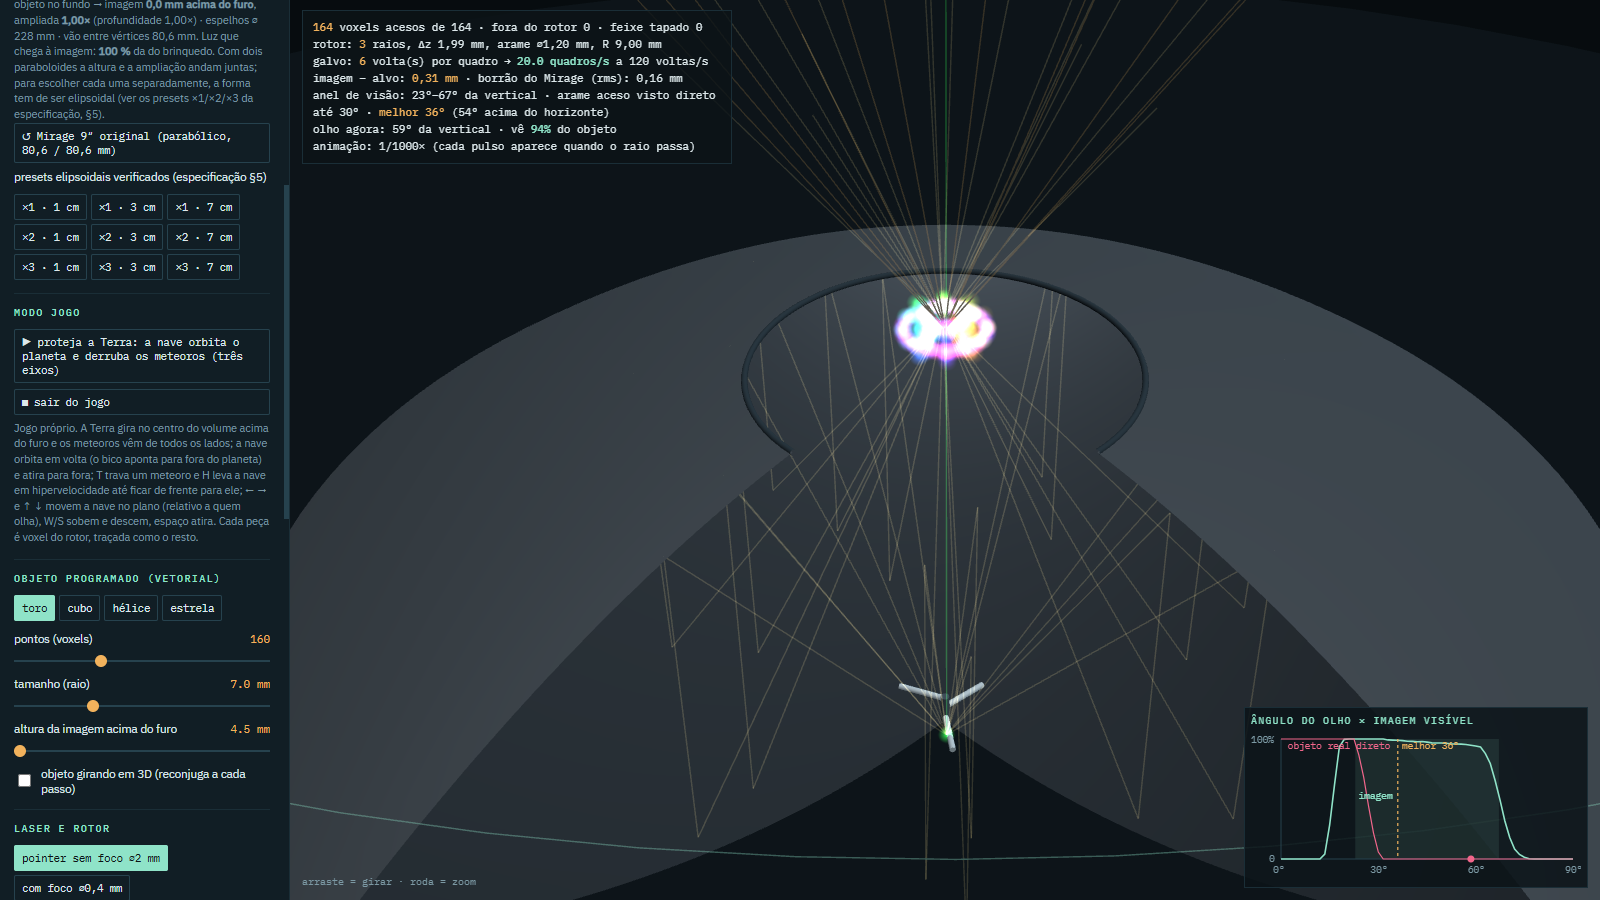
\includegraphics[width=\columnwidth]{mirage-rotor}
\caption{Aba ``rotor espiral'' do simulador principal: par parab\'olico do Mirage, rotor de arames no leito e galvan\^ometro no eixo. O toro acima do furo \'e formado por 164 voxels tra\c{c}ados (borr\~ao 0,16~mm rms); o gr\'afico mostra a fra\c{c}\~ao vis\'ivel da imagem por \^angulo do olho, com o melhor \^angulo marcado.}
\label{fig:rotor}
\end{figure}

\begin{figure}[t]
\centering
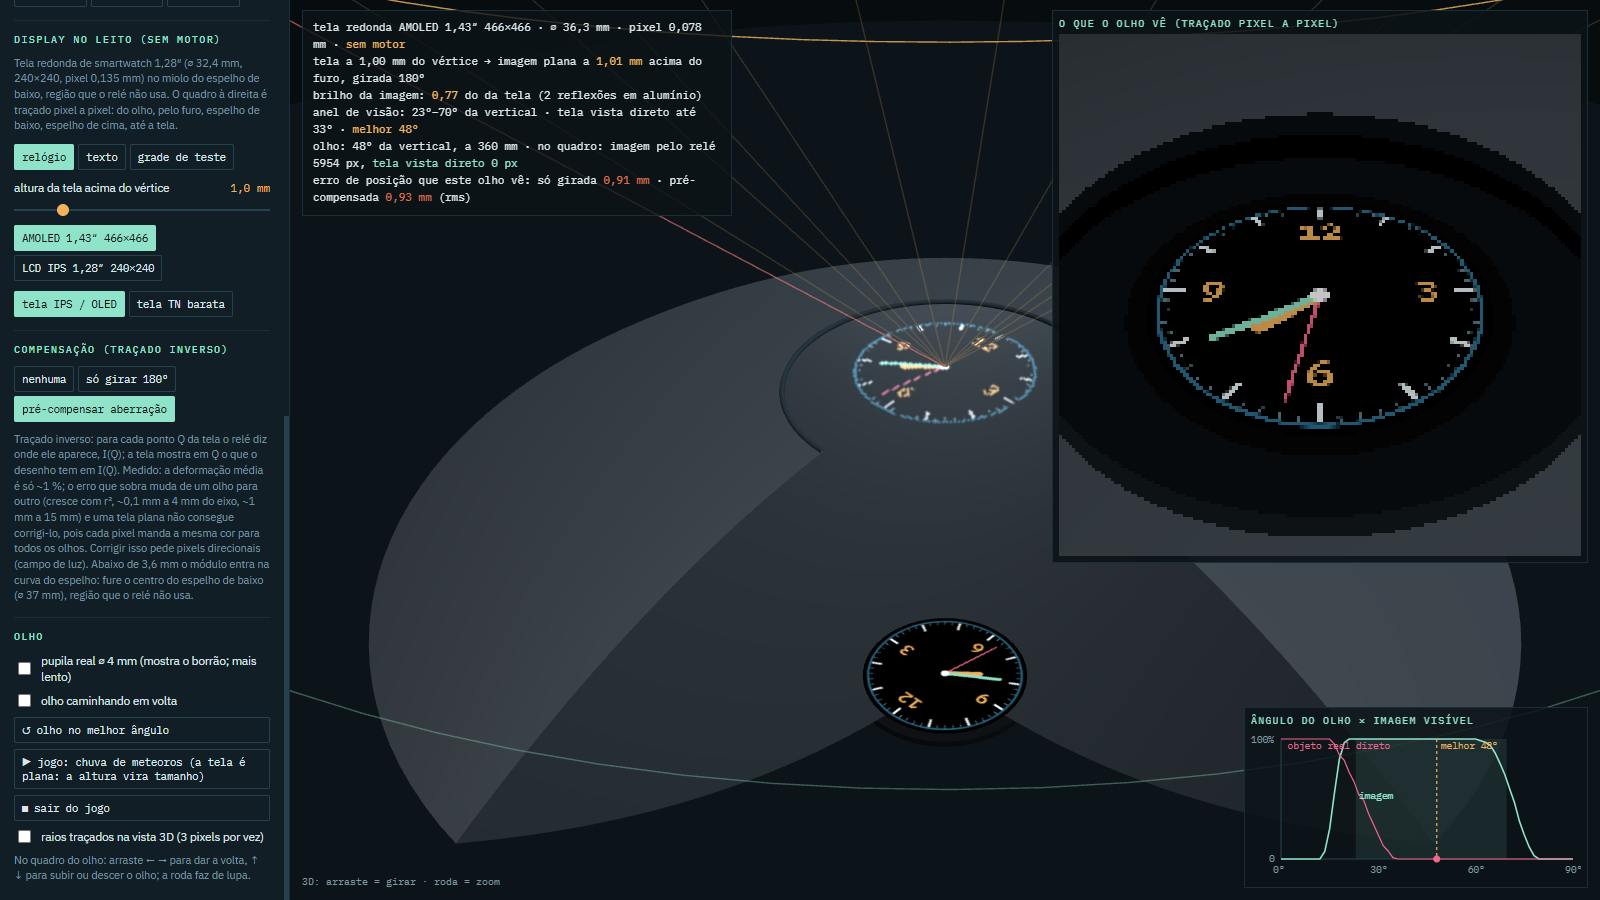
\includegraphics[width=\columnwidth]{mirage-display}
\caption{Aba ``display no leito'': tela redonda AMOLED (pixel 0,078~mm) no centro n\~ao usado do espelho inferior, sem motor. O quadro \`a direita \'e a vista do olho tra\c{c}ada pixel a pixel (olho $\to$ furo $\to$ espelho inferior $\to$ espelho superior $\to$ tela), com pr\'e-compensa\c{c}\~ao pelo mapa tra\c{c}ado.}
\label{fig:display}
\end{figure}

\begin{figure}[t]
\centering
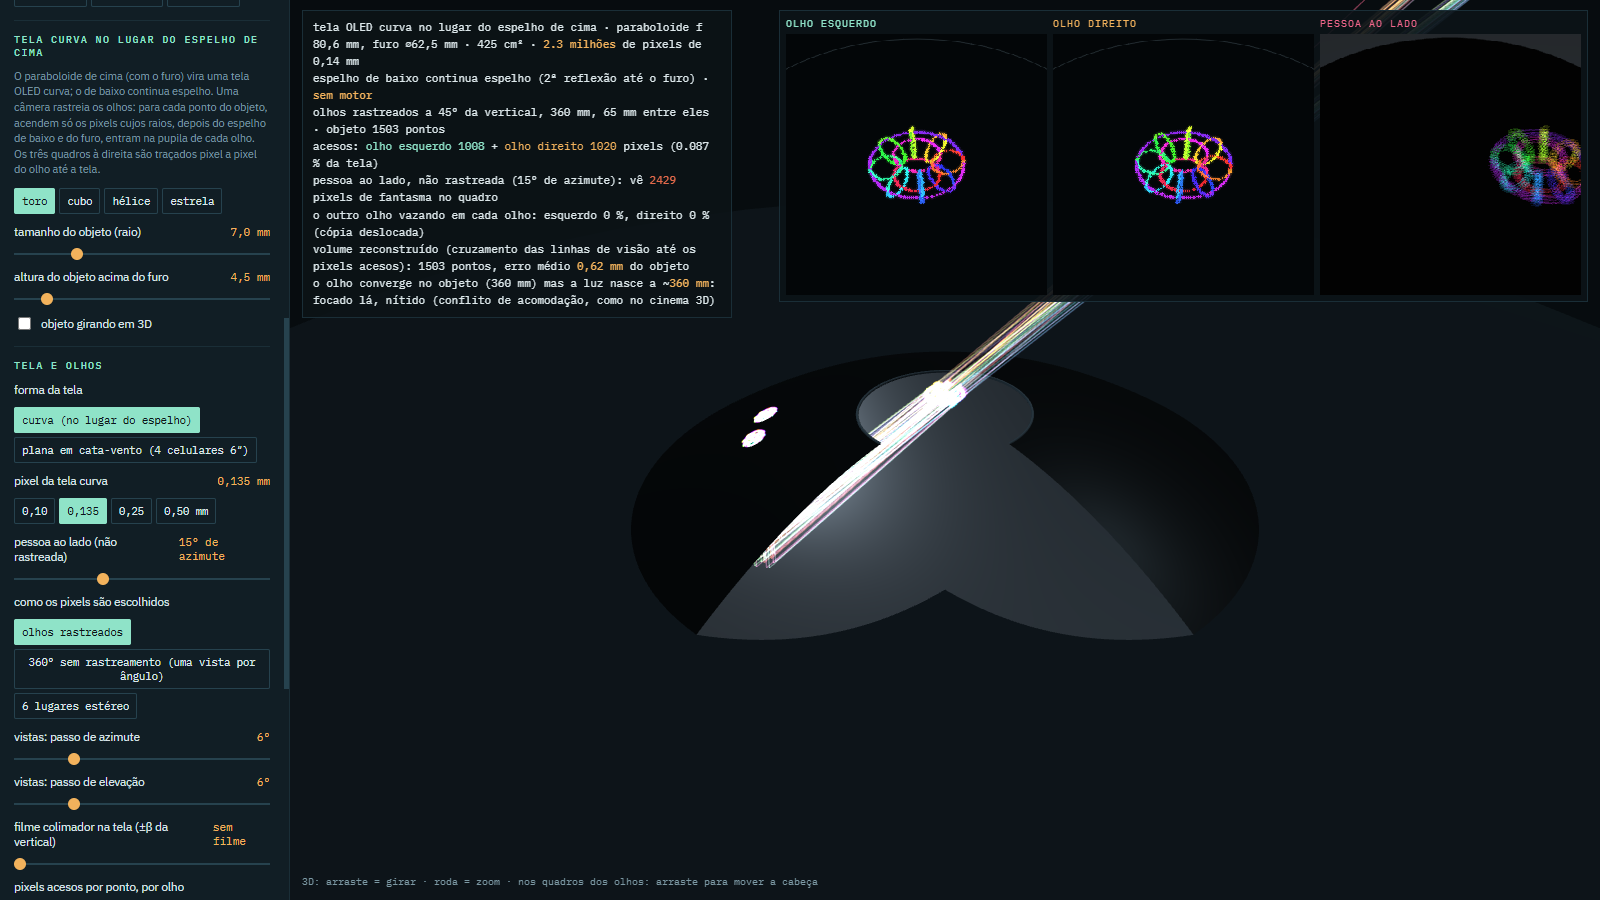
\includegraphics[width=\columnwidth]{mirage-parab}
\caption{Aba ``tela no espelho de cima'': o paraboloide superior vira um OLED curvo (2,3 milh\~oes de pixels de 0,14~mm) e o inferior continua espelho. Com olhos rastreados a 45$^\circ$, acendem-se 1008 + 1020 pixels (0,087~\% da tela); a pessoa ao lado, n\~ao rastreada, v\^e uma c\'opia deslocada (2429 pixels de fantasma).}
\label{fig:parab}
\end{figure}

\begin{figure}[t]
\centering
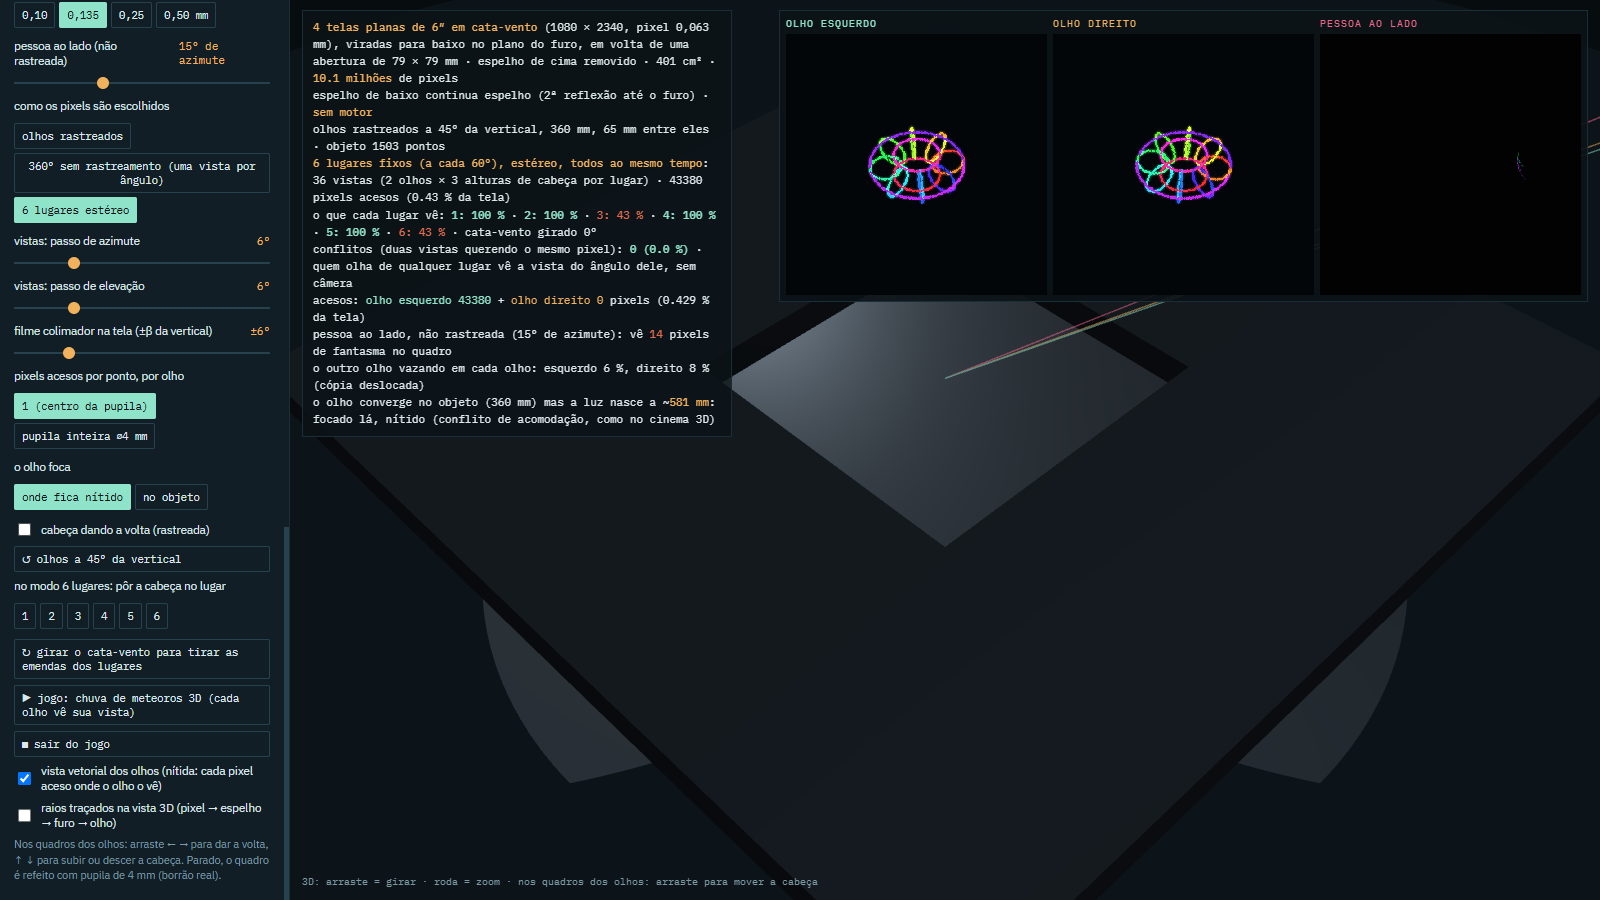
\includegraphics[width=\columnwidth]{mirage-petalas}
\caption{P\'etalas: quatro telas planas de 6 polegadas no plano focal, em cata-vento ao redor de uma abertura de 79$\times$79~mm, modo de seis lugares est\'ereo (36 vistas acesas, 0 conflitos). Sem girar o cata-vento, as costuras deixam os lugares 3 e 6 com 43~\%; o giro de 9$^\circ$ leva todos a 100~\%. A pessoa ao lado v\^e 14 pixels de fantasma.}
\label{fig:petalas}
\end{figure}

\paragraph{Rotor de voxels (Fig.~\ref{fig:rotor})} Um rotor espiral de arames foscos (uma volta, passo $\Delta z \le$ spot) gira no leito; um galvan\^ometro no eixo, 150~mm acima do furo, acende cada voxel quando a p\'a certa passa. \'E a fam\'ilia dos mostradores volum\'etricos de varredura~\cite{favalora2005,jones2007}, com a diferen\c{c}a de que a imagem \'e relayada pelo par. O agendamento vetorial (saltos proporcionais a $\Delta\theta$) d\'a $\approx$17--20 quadros/s para 110--160 voxels. A otimiza\c{c}\~ao com o tra\c{c}ado como custo --- recozimento para a ordem das p\'as~\cite{kirkpatrick1983}, Lloyd para as alturas~\cite{lloyd1982}, Gauss--Newton por voxel sobre 24 olhos num anel --- quase n\~ao mudou o erro: o res\'iduo \'e a aberra\c{c}\~ao do brinquedo fora do foco, por isso os objetos foram encolhidos para perto dele.

\paragraph{A escada helicoidal e o posicionamento de cada voxel (Fig.~\ref{fig:objetos})} O rotor \'e uma escada em h\'elice de $M$ p\'as de arame fosco, uma volta completa, com passo vertical $\Delta z$ igual ou menor que o di\^ametro do ponto do laser; cada voxel desejado \'e primeiro conjugado para o espa\c{c}o do objeto (Newton sobre o jacobiano paraxial do relay), depois atribu\'ido \`a p\'a cuja altura mais se aproxima da sua e \`a fase de rota\c{c}\~ao em que essa p\'a cruza o raio que passa pela sua posi\c{c}\~ao lateral; o ponto aceso fica no lado do arame voltado para o feixe. Voxels que coincidem no mesmo ponto da mesma p\'a compartilham um pulso. O cubo do eixo (di\^ametro ajust\'avel) \'e uma zona morta: perto dele as p\'as superiores atravessam o feixe, por isso objetos cheios ficam a mais de 0,8~mm do eixo e o feixe bloqueado \'e desviado para a p\'a vizinha (no m\'aximo $1{,}6\,\Delta z$ de erro extra em profundidade). Ordenar as p\'as por um passo \'aureo (``v\'ortice'') reduz os bloqueios perto do eixo ao pre\c{c}o de um pouco mais de oclus\~ao para o observador. A biblioteca de objetos vetoriais --- toro, cubo, h\'elice e estrela, al\'em de uma m\'ascara facial em relevo e do jogo --- redimensiona a escada a cada objeto: o cubo de 7~mm usa 21 p\'as com $\Delta z = 0{,}67$~mm e arame de 0,42~mm (156 voxels, 0,18~mm do alvo, 20~qps); a estrela, 11 p\'as com $\Delta z = 1{,}26$~mm (147/160 voxels acesos, 13 fora do rotor, 0,36~mm, 15~qps); o toro, 164 voxels a 0,16~mm.

\begin{figure*}[t]
\centering
\begin{minipage}[t]{0.325\textwidth}\centering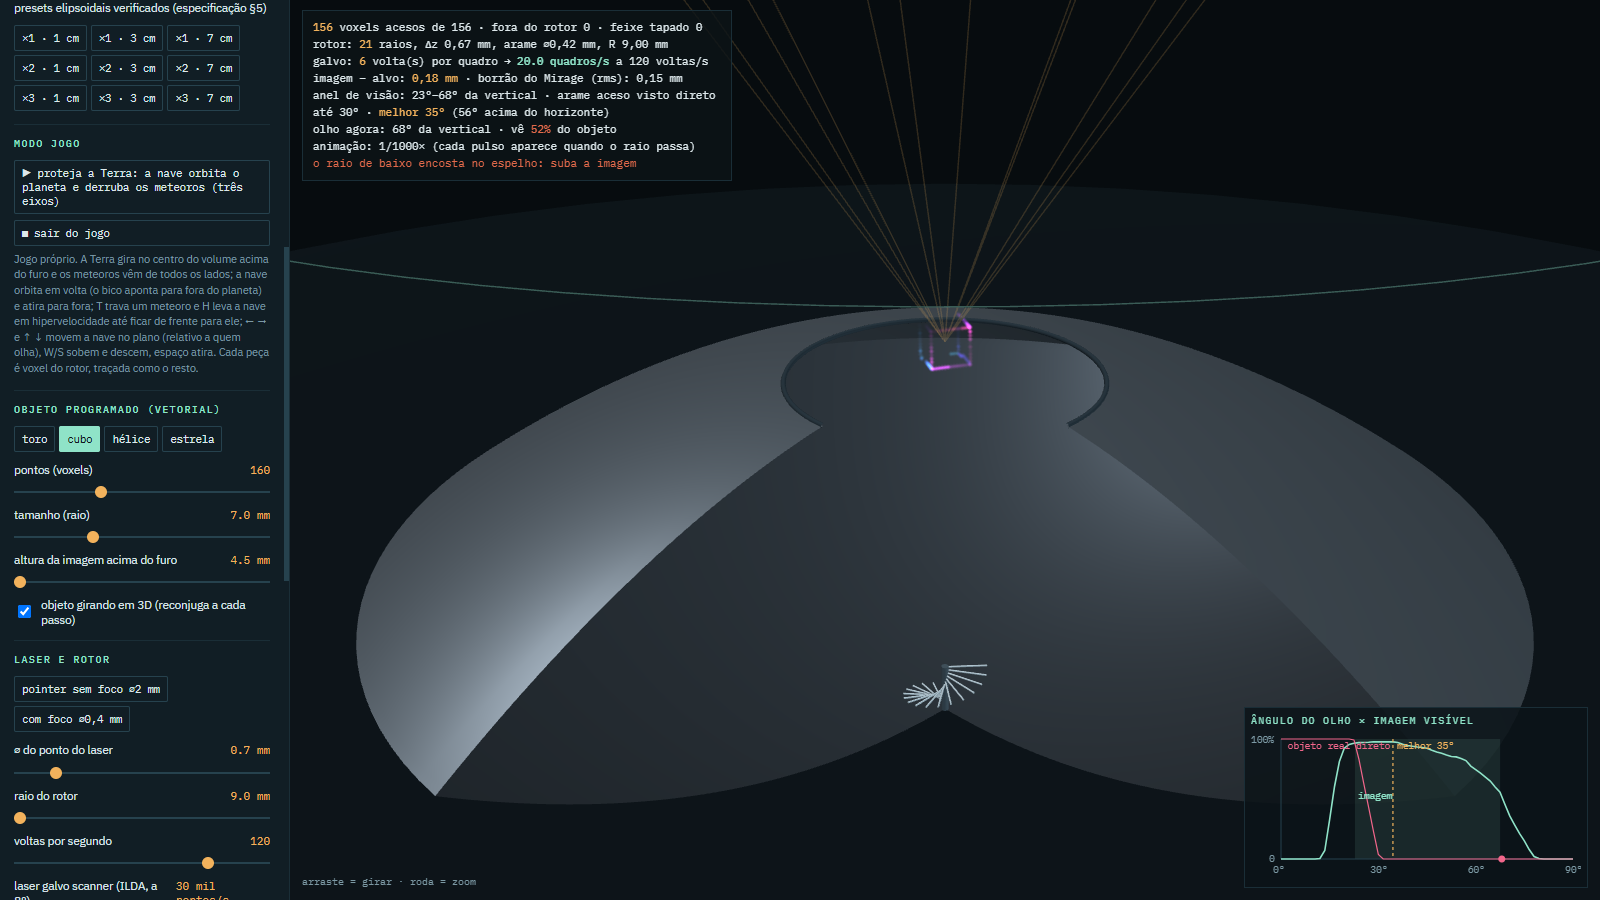
\includegraphics[width=\linewidth]{mirage-cubo}\end{minipage}\hfill
\begin{minipage}[t]{0.325\textwidth}\centering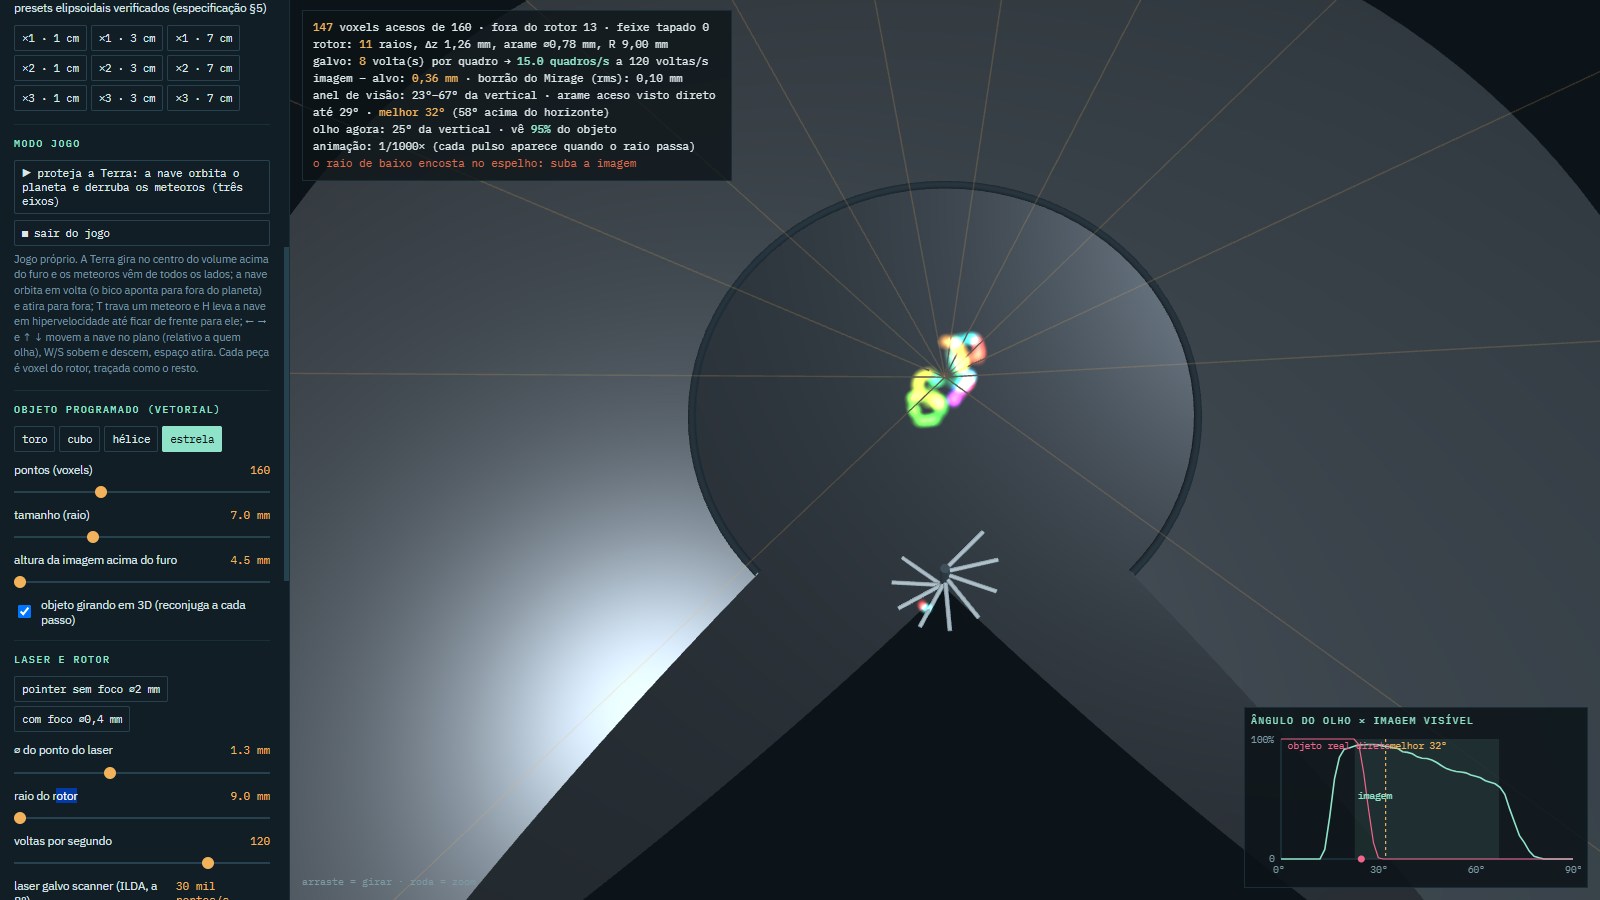
\includegraphics[width=\linewidth]{mirage-estrela}\end{minipage}\hfill
\begin{minipage}[t]{0.325\textwidth}\centering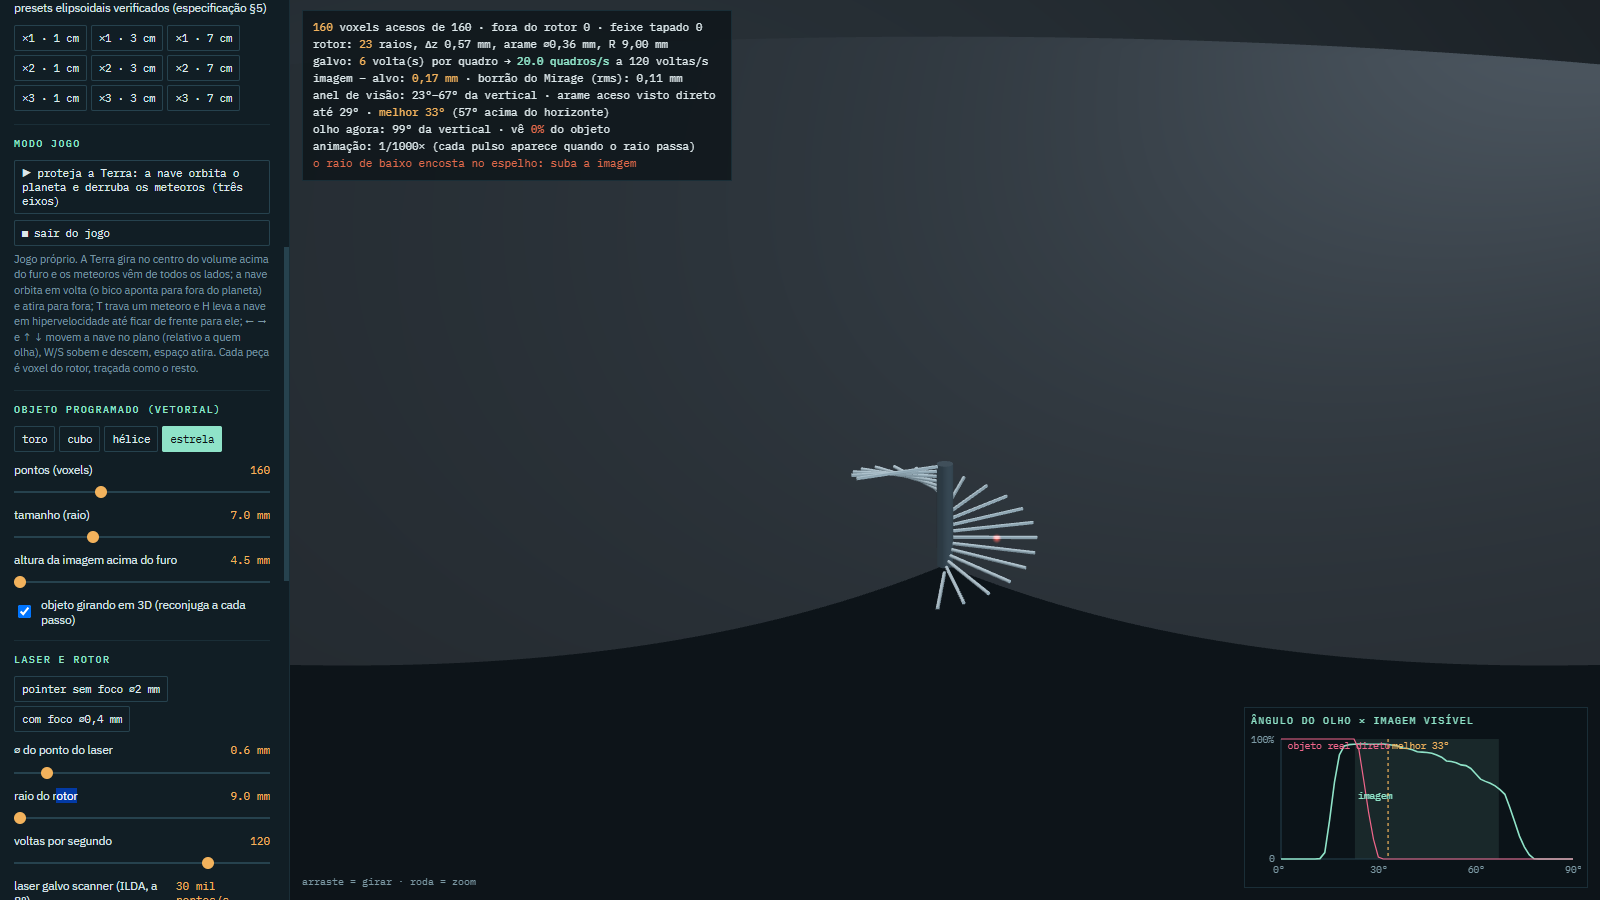
\includegraphics[width=\linewidth]{mirage-helice}\end{minipage}
\caption{Objetos vetoriais no rotor. Esquerda: cubo de 7~mm (21 p\'as, $\Delta z$ 0,67~mm, 156 voxels, 0,18~mm do alvo, 20~qps), com o objeto girando em 3D e reconjugado a cada passo. Centro: estrela (11 p\'as, $\Delta z$ 1,26~mm, 147/160 voxels, 15~qps). Direita: a escada helicoidal de arames vista de perto no leito do espelho inferior, com o ponto aceso de um pulso e os raios do galvo.}
\label{fig:objetos}
\end{figure*}

\paragraph{Telas no lugar dos espelhos (Figs.~\ref{fig:display} e \ref{fig:parab})} O display plano no leito dispensa o motor, mas a corre\c{c}\~ao por mapa tra\c{c}ado s\'o remove o erro m\'edio; o res\'iduo depende da posi\c{c}\~ao do olho e cresce com $r^2$. Um display no lugar do espelho inferior n\~ao forma imagem: a maior parte da luz volta \`a pr\'opria tela. No lugar do espelho superior, um OLED curvo fica perto do plano focal do espelho inferior, de modo que cada pixel mapeia uma dire\c{c}\~ao ($\approx$1,65~mm por grau acima do furo); com rastreio ocular, um pixel por ponto e por olho d\'a vistas est\'ereo n\'itidas, com 6~\% de vazamento e uma c\'opia deslocada para quem n\~ao \'e rastreado. Sem rastreio, zonas fixas com filme colimador trocam duplica\c{c}\~ao por fragmenta\c{c}\~ao; seis assentos fixos (duas alturas de olho, tr\^es de cabe\c{c}a) acendem 36 zonas sem conflito usando 0,65~\% da tela. Multiplexar os assentos no tempo \'e desnecess\'ario --- eles n\~ao compartilham pixels --- e custaria cintila\c{c}\~ao.

\paragraph{P\'etalas (Fig.~\ref{fig:petalas})} Quatro pain\'eis planos de 6 polegadas no plano focal, em cata-vento ao redor de uma abertura de 79~mm, superam o OLED curvo em todas as m\'etricas (0,20 vs 0,60~mm; vazamento 0 vs 6~\%; fantasma 2 vs 434 pixels). As costuras das molduras custam vistas em faixas de azimute de 24--33$^\circ$ e 39--48$^\circ$ (m\'odulo 90$^\circ$); girar o cata-vento 9$^\circ$ leva os seis assentos a 100~\% de cobertura.

\paragraph{Concavidade e amplia\c{c}\~ao} Com paraboloides, altura e amplia\c{c}\~ao andam juntas; com o furo do brinquedo, $\times2$ deixa passar 35~\% da luz e $\times3$ apenas 17~\%. A amplia\c{c}\~ao sem distor\c{c}\~ao vem do par elipsoidal estigm\'atico da especifica\c{c}\~ao: os presets $\times1$, $\times2$ e $\times3$ reproduziram no simulador os di\^ametros, o furo e os aumentos previstos (1,000 / 1,998 / 2,998), com imagem ereta --- ao contr\'ario do giro de 180$^\circ$ do par parab\'olico.

\paragraph{Um jogo como teste de carga} Para provar que a cadeia tra\c{c}ada sustenta conte\'udo interativo, foi desenvolvido um jogo original, \lq\lq Proteja a Terra\rq\rq: um globo procedural gira no centro do volume, meteoros chegam da borda do cubo de jogo, uma nave orbita o planeta (nariz radial, tr\^es eixos de movimento), trava alvos (tecla T), salta em hipervelocidade por um arco de c\'irculo m\'aximo (H) e dispara pela dire\c{c}\~ao de intercepta\c{c}\~ao; h\'a trilha e efeitos sonoros sintetizados. O jogo roda nas tr\^es abas do par e na aba do acess\'orio, sempre \emph{atrav\'es} do tra\c{c}ado: no rotor cada pe\c{c}a vira voxels reconjugados a cada 0,1~s ($\approx$66--110 voxels, galvo a $\approx$17~qps); na tela do leito \'e desenhado em perspectiva e mapeado pela tela; no espelho superior cada olho ou assento recebe apenas os pixels que veria ($\approx$14\,000 pontos de superf\'icie, 2$\times$4\,200 pixels, 79~qps); no acess\'orio \'e refeito pelos dois olhos acima da abertura (57~qps). Em nenhum lugar o jogo \'e desenhado diretamente na imagem.

\section{Recorte c\^oncavo e tela larga}
\label{sec:recorte}
A passagem para um \'unico espelho come\c{c}ou com um recorte retangular de esfera ($R = 700$~mm, 520$\times$300~mm) e um tablet de 10,1 polegadas abaixo do eixo, voltado para o espelho. Medimos: imagem de 199$\times$128~mm flutuando a 685~mm do espelho, borr\~ao de 0,14~mm na pupila de 4~mm e um bojo (curvatura mais trap\'ezio) de $\approx$8~mm visto pelo olho. Ampliar o recorte para 800$\times$500~mm n\~ao muda a imagem, mas alarga a janela de onde ela \'e vista inteira de 140$\times$60 para 540$\times$260~mm --- o recorte compra janela, n\~ao imagem. Aproximar a tela ($u = 600$~mm) d\'a 1,16$\times$ a 796~mm, mas eleva o bojo a $\approx$19~mm e encolhe a janela. A pr\'e-compensa\c{c}\~ao tra\c{c}ada (pontos aparentes numa grade 41$\times$25, maior ret\^angulo inscrito, tabela por pixel) reduz o res\'iduo de 8,3 para 0,0~mm no olho de projeto. Um gabinete em forma de console, cuja abertura \'e dimensionada pelos pr\'oprios feixes tra\c{c}ados, esconde o espelho: frente a 377~mm, abertura de 546$\times$337~mm, imagem 308~mm para fora dela, fundo com 1,7~\% do branco da imagem (vidro fum\^e e interior preto). O jogo do simulador principal foi portado e desenhado em perspectiva na tela, atualizado a cada 0,08~s. Esta etapa validou tr\^es ferramentas que o acess\'orio herdou --- ponto aparente por Newton, pr\'e-compensa\c{c}\~ao por olho e gabinete tra\c{c}ado --- mas, com $\approx$0,3~m$^3$ de m\'ovel, n\~ao \'e port\'atil. Fica tamb\'em o seu limite: s\'o um olho foi medido; a an\'alise binocular da Se\c{c}\~ao~\ref{sec:evol} mostra que a imagem real de uma tela plana n\~ao d\'a profundidade pr\'opria, o que vale igualmente aqui.

\section{Sequ\^encia de tentativas do acess\'orio}
\label{sec:evol}
A Tabela~\ref{tab:evol} resume a evolu\c{c}\~ao. Cada linha \'e uma hip\'otese que o tra\c{c}ado confirmou ou refutou; as se\c{c}\~oes seguintes detalham as que mudaram o rumo.

\begin{table*}[t]
\centering
\caption{Evolu\c{c}\~ao das tentativas e principal medida de cada uma (tra\c{c}ado de raios). ``Compart.'' = pixels usados pelos dois olhos; VAC = conflito verg\^encia--acomoda\c{c}\~ao.}
\label{tab:evol}
\small
\begin{tabular}{@{}lp{6.2cm}p{6.2cm}p{3.2cm}@{}}
\toprule
\# & Arranjo & Medida decisiva & Veredito \\
\midrule
1 & Par Mirage + rotor espiral de arames + galvo & RMS do voxel 0,28~mm (spot 2~mm); treino 0,67$\to$0,60~mm & volume real, mas motor e laser \\
2 & Display plano no leito do par & distor\c{c}\~ao m\'edia 1~\%, res\'iduo $\propto r^2$ (0,09$\to$1,1~mm) & sem motor, sem volume \\
3 & Display no lugar do espelho inferior & 75--86~\% da luz volta \`a tela; nenhuma imagem & refutado \\
4 & OLED curvo no lugar do espelho superior, olho rastreado & 0,6~mm; vazamento 6~\%; foco a 575 vs 360~mm & est\'ereo, VAC \\
5 & Quatro telas planas no plano focal (``p\'etalas'') & 0,20~mm; vazamento 0; 6 assentos 100~\% (giro 9$^\circ$) & melhor da fam\'ilia Mirage \\
6 & Recorte largo de esfera ($R$ 700) + tablet & imagem 199$\times$128~mm a 685~mm; borr\~ao 0,14; bojo 8,3$\to$0,0~mm & grande, n\~ao port\'atil \\
7 & Meia-lua do Mirage ($R_v$ 127) + celular de 6,5\,\textquotedbl, abertura ao p\'e & 40~\% da tela; 5,6~L & port\'atil, tela parcial \\
8 & Tela inteira (fatia 180$\times$366) & 35/35 pontos; ret\^angulo limpo 46$\times$99~mm; 14,6~L & completa, curva \\
9 & Pixel a pixel (li\c{c}\~ao da aba 3) & 46$\to$69~cm$^2$ sem mudar o aparelho & ganho gr\'atis \\
10 & Dois olhos na imagem real & 1,1 / 3,2 / 3,6~mm por olho & sem profundidade pr\'opria \\
11 & Telefone no foco, abertura 56~mm & compart. 0~\%; erro 0,71~mm; cabe\c{c}a $\pm$60~mm & profundidade real \\
12 & Paisagem + abertura 72$\times$56 & cabe\c{c}a $\pm$120~mm; compart. 1--2~\% & mais paralaxe \\
13 & Cata-vento (abertura no eixo) & borr\~ao 2,3~mm & refutado \\
14 & Telefone de p\'e + vidro 45$^\circ$ & borr\~ao 0,73~mm; 1,9~L; brilho 25~\% & n\'itido, escuro \\
15 & Telefone deitado cobrindo o foco, 88,5$^\circ$ & borr\~ao 0,71~mm; brilho 100~\%; 4,3~L & n\'itido \\
16 & Espelho tamb\'em sob a abertura (``melhor dos mundos'') & 35/35; 48/49 bin.; janela 220$\times$720; 11,7~L & tela inteira, plana \\
17 & Mesmo espelho, telefone no foco, duas imagens & 27/27; erro 0,81; borr\~ao 1,34; 5,2~L & volume em caixa baixa \\
18 & Fatia Mirage inclinada 16$^\circ$ + iPhone 15 Pro & erro 0,65 (pior 1,42); borr\~ao 0,77; 72,5$^\circ$; $\pm$75~mm & configura\c{c}\~ao final \\
\bottomrule
\end{tabular}
\end{table*}

\subsection{Heran\c{c}a do par (linhas 1--5)}
As cinco primeiras linhas s\~ao as t\'ecnicas da Se\c{c}\~ao~\ref{sec:mirage}. Delas o acess\'orio herdou duas conclus\~oes: o res\'iduo de um relay parab\'olico \'e a aberra\c{c}\~ao fora de foco, e a \'unica forma de separar pixels por olho com telas comuns \'e p\^o-las no plano focal atr\'as de uma abertura menor que a dist\^ancia interocular.

\subsection{O acess\'orio port\'atil (linhas 6--10)}
Com um celular de 6,5\,\textquotedbl{} e a meia-lua do Mirage (di\^ametro 180~mm, $R_v = 127$~mm) numa caixa de 5,6~L, apenas 40~\% da tela \'e vis\'ivel: a imagem real \'e maior que a tela e o espelho, mais distante do olho, parece menor que ela (Fig.~\ref{fig:meialua}). Ver a tela inteira exigiu uma fatia de 180$\times$366~mm e 14,6~L, e mesmo assim o ret\^angulo sem curvatura tinha 46$\times$99~mm. O modo pixel a pixel recuperou 69~cm$^2$ sem tocar no aparelho; um recozimento com semente fixa, $R_v$ preso a $2\times80{,}6$~mm e custo binocular, chegou a 88~cm$^2$ em 9,5~L (Fig.~\ref{fig:aprendido}).

\begin{figure}[t]
\centering
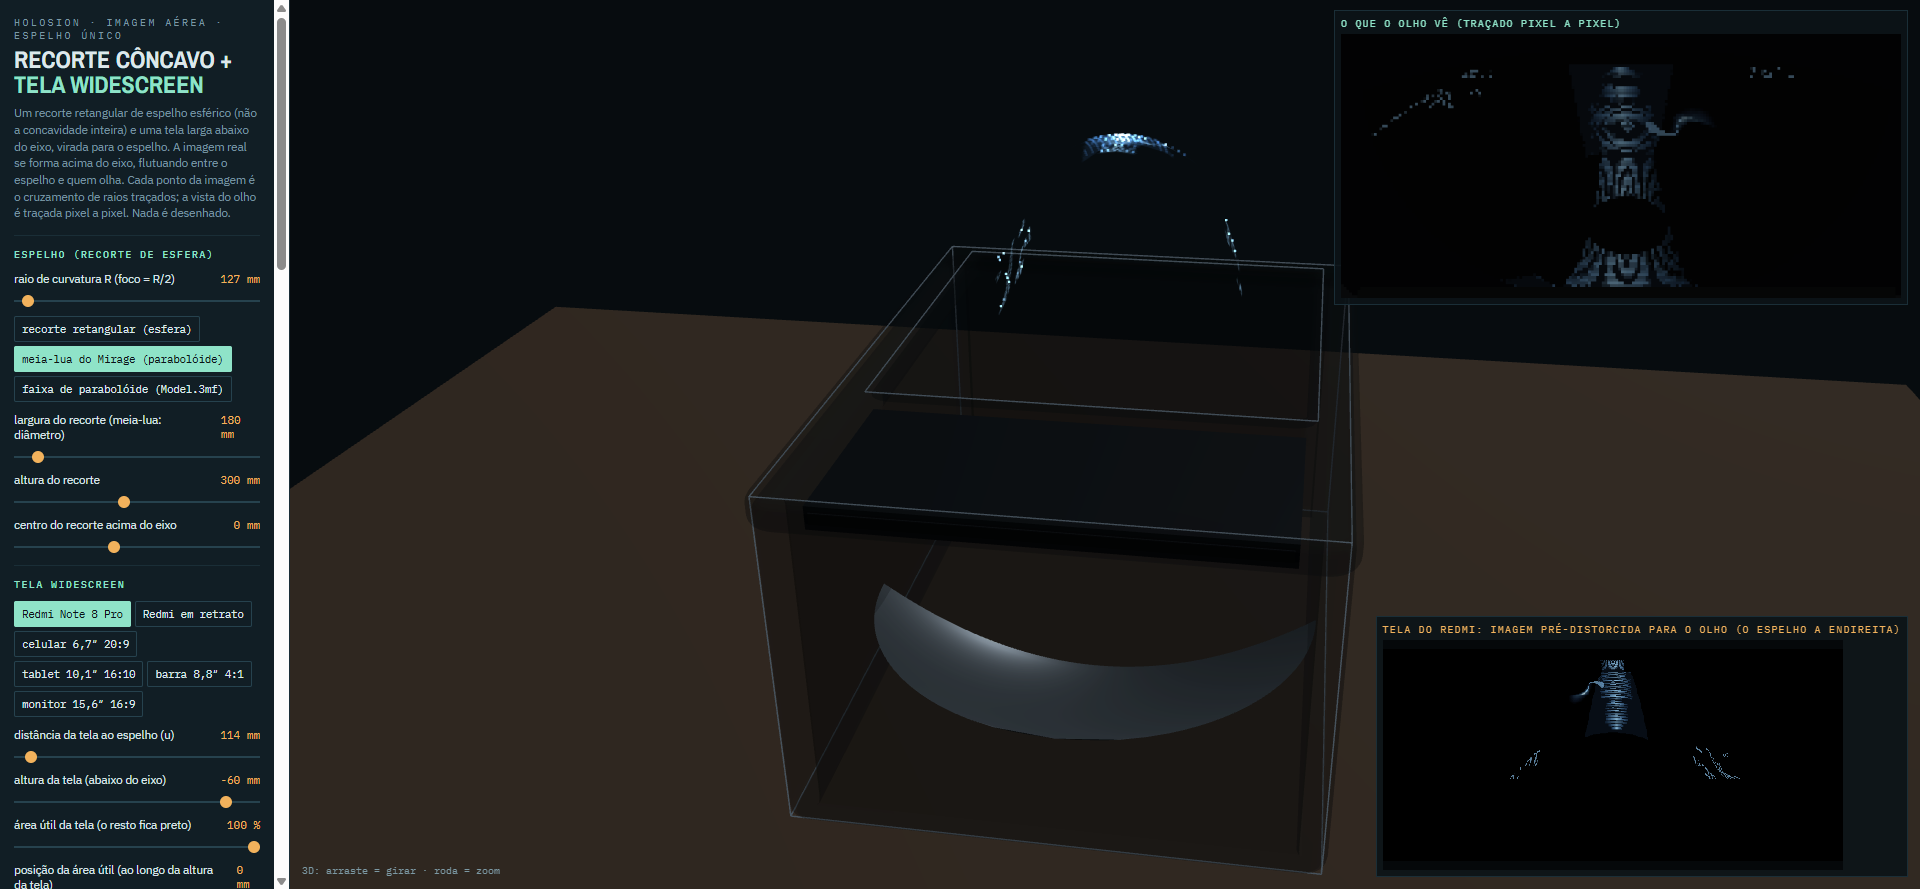
\includegraphics[width=\columnwidth]{meialua}
\caption{Meia-lua do Mirage sob o telefone deitado, abertura ao p\'e dele. A imagem real (pontos) flutua 61~mm acima do tampo; o olho v\^e apenas uma fra\c{c}\~ao da tela.}
\label{fig:meialua}
\end{figure}

\begin{figure}[t]
\centering
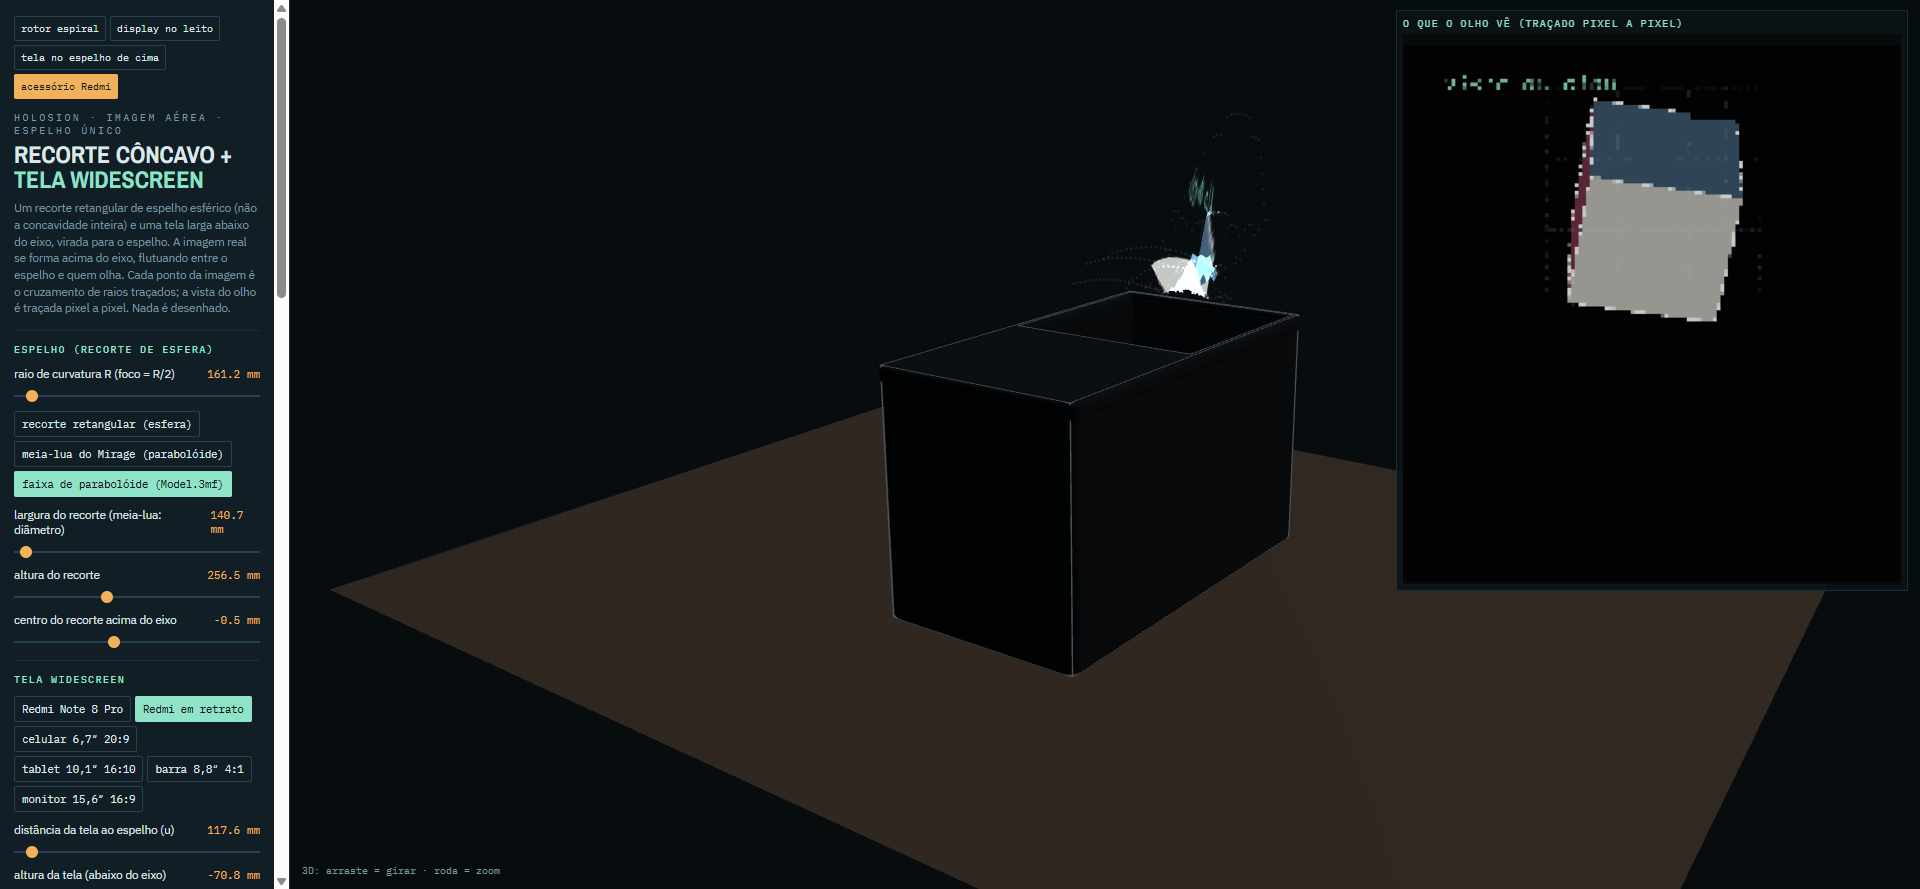
\includegraphics[width=\columnwidth]{aprendido}
\caption{Resultado do recozimento simulado sobre a fatia do Mirage (custo = \'area projetada $-$ litros $-$ penalidades). O quadro \`a direita \'e a vista tra\c{c}ada do olho.}
\label{fig:aprendido}
\end{figure}

A medida binocular encerrou essa linha: na imagem real os dois olhos veem os mesmos pixels, e a l\^amina imagem \'e inclinada (26~mm de profundidade ao longo da vista, 36$^\circ$); compensar para o olho m\'edio deixa cada olho 1,1 a 3,6~mm fora do lugar. O conte\'udo n\~ao tem profundidade pr\'opria.

\subsection{Est\'ereo no foco (linhas 11--15)}
Descendo o telefone ao plano focal e fechando a abertura a 56~mm, cada pixel chega a um olho s\'o (0~\% compartilhados) e os dois olhos reconstroem um cubo de 30~mm com 0,71~mm de erro (Fig.~\ref{fig:estereo}). O pre\c{c}o: cada olho usa uma mancha de $\approx$15$\times$16~mm da tela, pr\'e-distorcida em trap\'ezio (Fig.~\ref{fig:duas}), e a luz chega focada no infinito enquanto os olhos convergem a 420~mm --- um conflito de 2,0~D no tampo a 4,3~D a 220~mm acima dele~\cite{hoffman2008}. O volume onde h\'a profundidade vai de 40~mm dentro da caixa a $\approx$200~mm acima do tampo, encolhendo de 72$\times$56 para 8$\times$24~mm (Fig.~\ref{fig:volume}). O telefone em paisagem com abertura 72$\times$56~mm dobrou a excurs\~ao da cabe\c{c}a para $\pm$120~mm (Fig.~\ref{fig:paralaxe}).

O olhar precisa ser quase vertical: a 75$^\circ$ os feixes saem 15$^\circ$ fora do eixo, o mapa dire\c{c}\~ao$\to$pixel dobra e cada olho v\^e o cubo duplicado; a 86--88,5$^\circ$ o erro cai para 0,7~mm. O arranjo tipo cata-vento (abertura no eixo, telefone no foco ao lado) borra 2,3~mm porque seus pixels ficam 40--116~mm fora do centro do foco. Um vidro semiespelhado a 45$^\circ$~\cite{pepper1890}, com o telefone de p\'e, p\~oe a tela virtualmente no foco sobre o eixo: borr\~ao de 0,73~mm em 1,9~L, mas com um quarto do brilho. O mesmo borr\~ao se obt\'em sem o vidro, com o telefone deitado cobrindo o foco e a abertura ao lado (0,71~mm, brilho total, 4,3~L).

\begin{figure}[t]
\centering
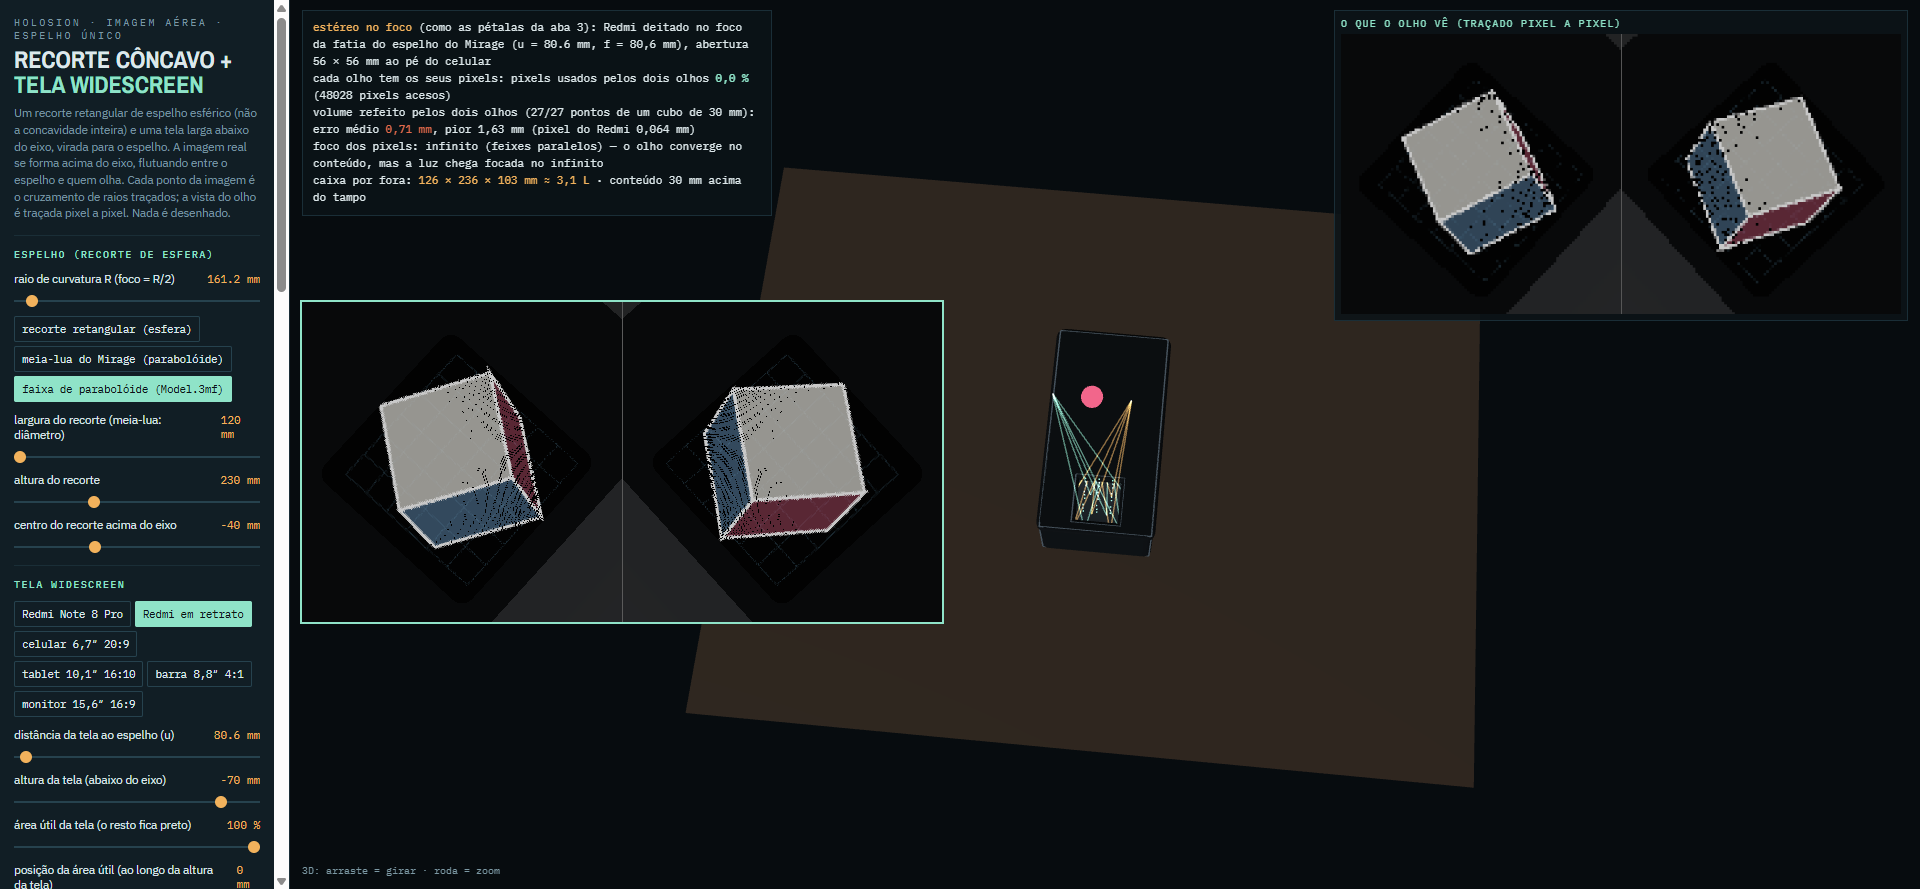
\includegraphics[width=\columnwidth]{estereo}
\caption{Est\'ereo no foco: olho esquerdo e olho direito tra\c{c}ados pixel a pixel, cada um pelos seus pr\'oprios pixels. Os pontos sobre a abertura s\~ao o cubo refeito pelo cruzamento das linhas de visada.}
\label{fig:estereo}
\end{figure}

\begin{figure}[t]
\centering
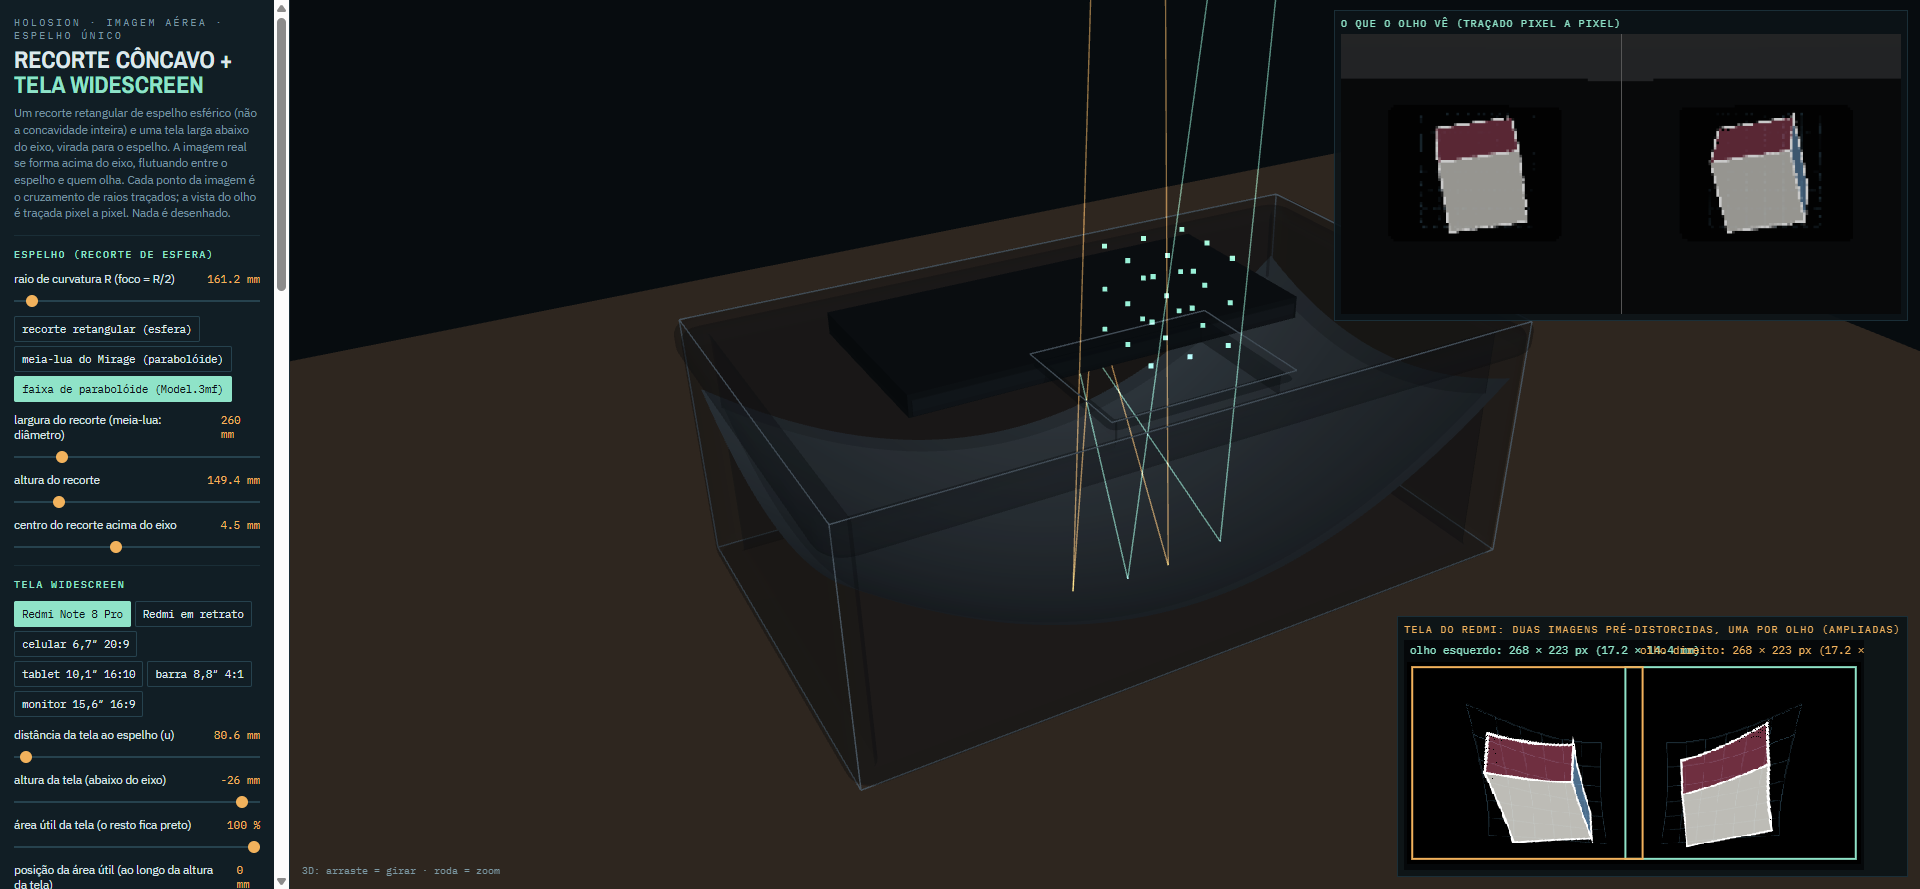
\includegraphics[width=\columnwidth]{duasimagens}
\caption{Caixa semitransparente e, embaixo \`a direita, as duas imagens pr\'e-distorcidas que o telefone exibe (uma por olho, $\approx$17$\times$14~mm cada).}
\label{fig:duas}
\end{figure}

\begin{figure}[t]
\centering
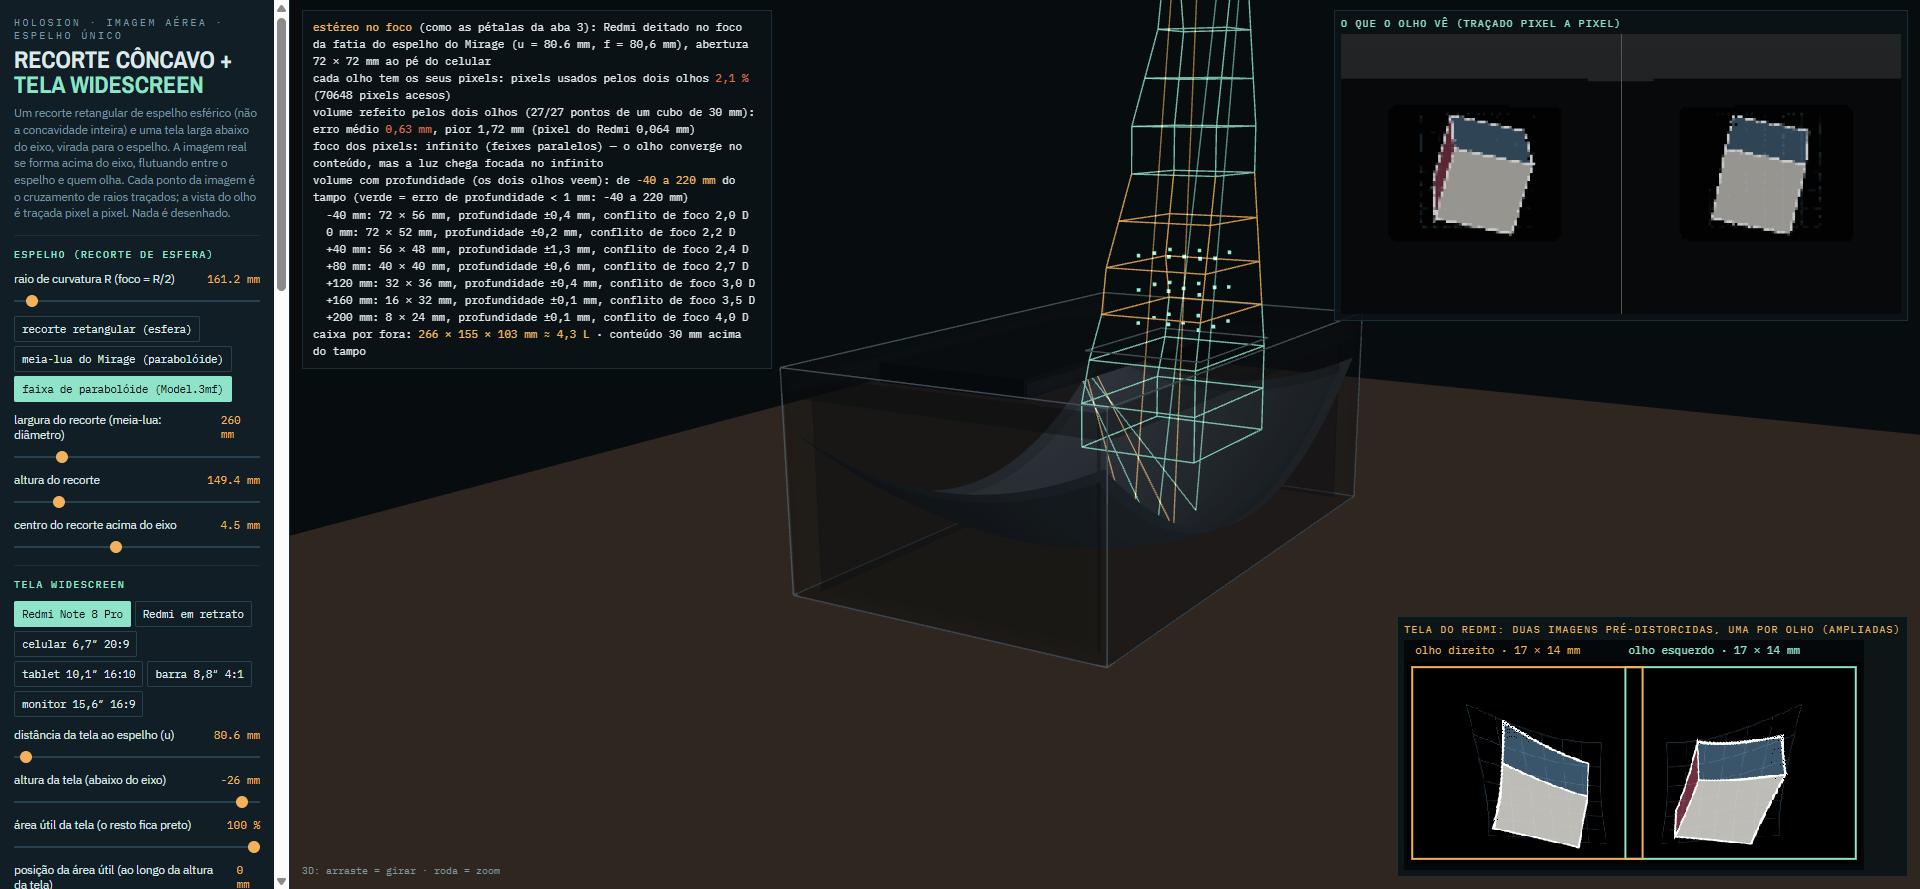
\includegraphics[width=\columnwidth]{volume}
\caption{Camadas do volume em que os dois olhos veem o mesmo ponto (verde: erro de profundidade $<1$~mm). O conflito de foco cresce de 2,0~D no tampo a 4,3~D no topo.}
\label{fig:volume}
\end{figure}

\begin{figure}[t]
\centering
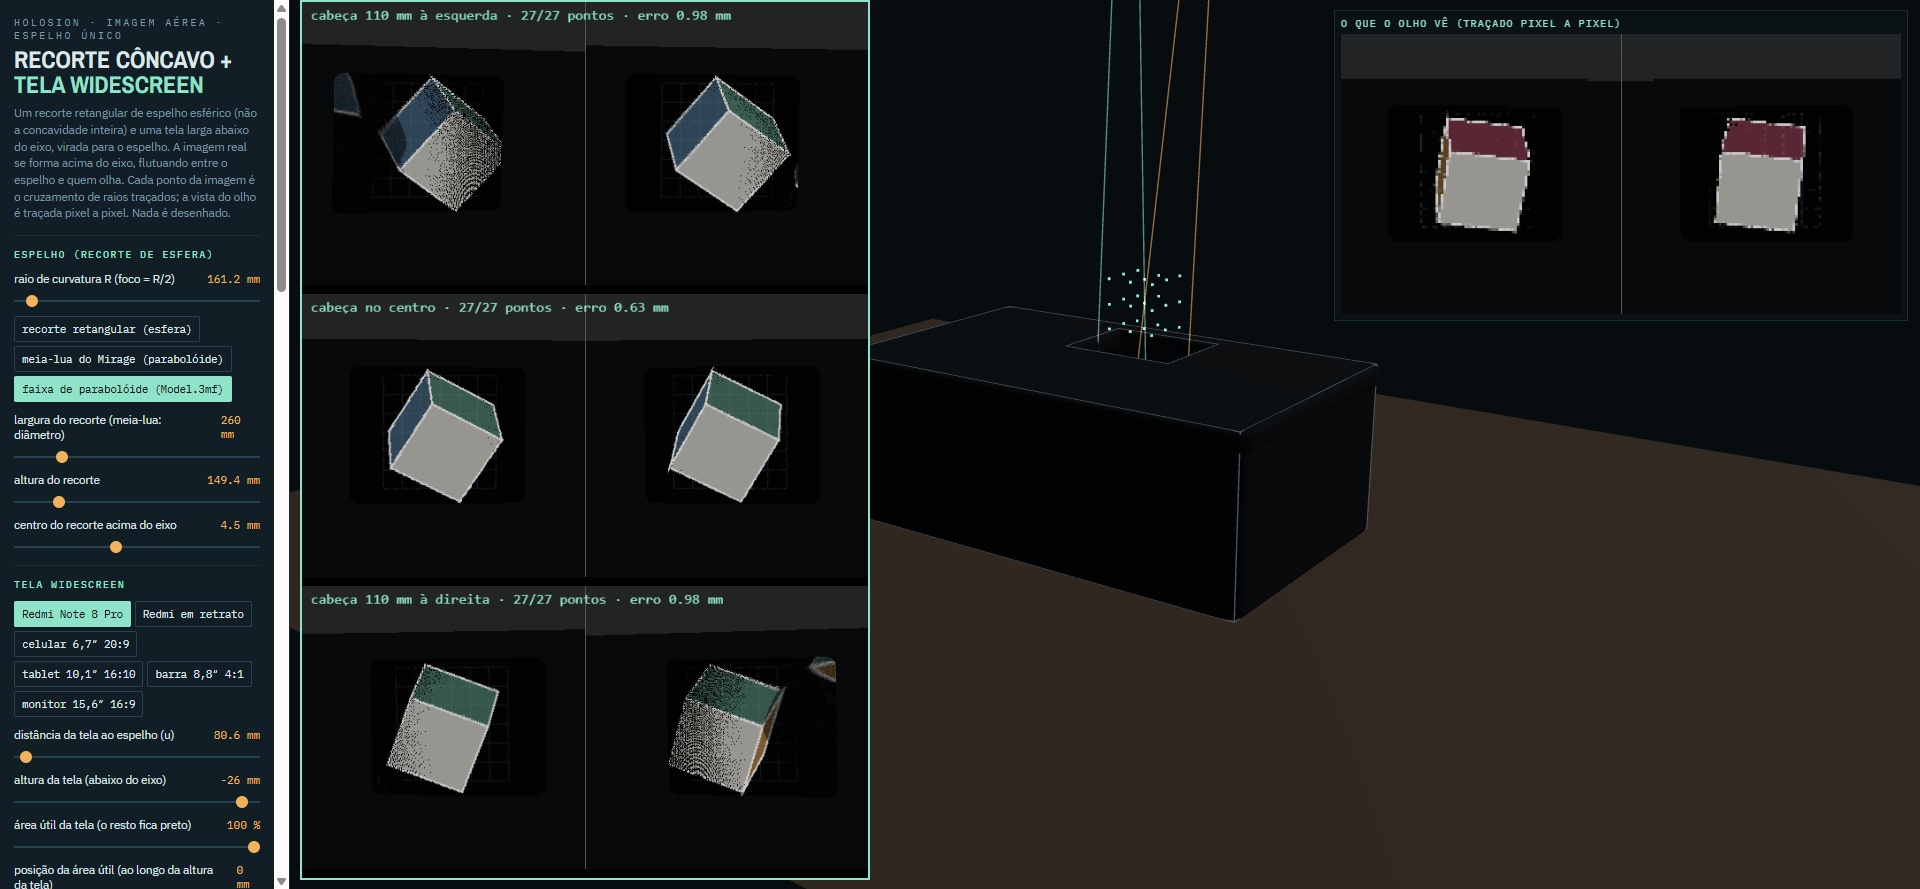
\includegraphics[width=\columnwidth]{paralaxe}
\caption{Telefone em paisagem, abertura 72$\times$56~mm: vistas dos dois olhos com a cabe\c{c}a 110~mm \`a esquerda, no centro e 110~mm \`a direita. Os 27 pontos do cubo s\~ao refeitos nas tr\^es posi\c{c}\~oes.}
\label{fig:paralaxe}
\end{figure}

\subsection{Tela inteira versus volume (linhas 16--17)}
Com a meia-lua \emph{sob} o telefone --- a disposi\c{c}\~ao do desenho original --- aumentar o espelho s\'o do lado do telefone piora (9 $\to$ 1--3 pontos vistos em 55--125~L): os pontos do espelho que mostrariam o resto da tela ficam sob a abertura e al\'em dela. Estendendo a mesma curvatura por todo o fundo da caixa, cortada pelas paredes e pela tampa, e afastando o telefone para 150~mm, o olho m\'edio v\^e 35/35 pontos, os dois olhos 48/49, com janela de observa\c{c}\~ao de 220$\times$720~mm, imagem de 124$\times$73~mm ($m = 0{,}82$) a 27~mm do tampo e borr\~ao de 0,64~mm, em 11,7~L (Fig.~\ref{fig:melhor}). O mesmo espelho com o telefone no foco ($u = f = 63{,}5$~mm) d\'a volume real em 5,2~L, com borr\~ao de 1,34~mm --- o dobro do obtido com $f = 80{,}6$~mm.

\begin{figure}[t]
\centering
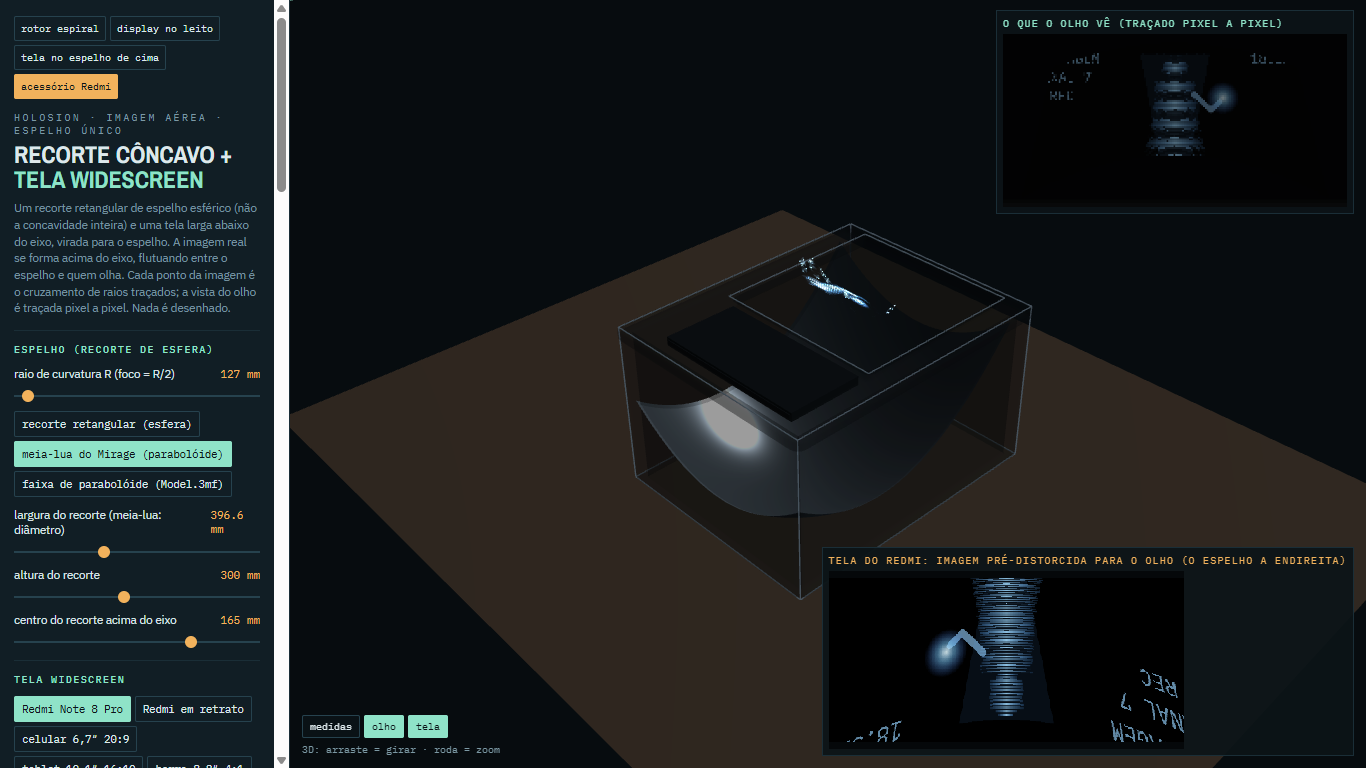
\includegraphics[width=\columnwidth]{melhor}
\caption{``Melhor dos mundos'': o espelho do Mirage ($R_v$ 127) cobre o fundo, sob o telefone e sob a abertura. O olho v\^e a tela inteira; o conte\'udo, por\'em, n\~ao tem profundidade pr\'opria.}
\label{fig:melhor}
\end{figure}

\subsection{Inclina\c{c}\~ao, pixel e aparelho (linha 18)}
Inclinar o espelho com o telefone parado desfoca; alterar s\'o a profundidade do v\'ertice borra 5--7~mm. Com o telefone deitado acompanhando o novo foco ($u = f\cos a$), o piso de borr\~ao permanece em $\approx$0,75~mm ($f = 80{,}6$) ou $\approx$1,0~mm ($f = 63{,}5$) para qualquer inclina\c{c}\~ao, mas o \^angulo de observa\c{c}\~ao desce de 88,5$^\circ$ para 72,5$^\circ$ a 16$^\circ$ de inclina\c{c}\~ao. Variar apenas o tamanho do pixel (0,13 / 0,064 / 0,032 / 0,016~mm) move o erro de profundidade (1,54 / 0,73 / 0,36 / 0,24~mm) e deixa o borr\~ao em 0,77~mm: a tela governa a precis\~ao, o espelho governa a nitidez. O iPhone~15~Pro (0,055~mm) melhora o pior ponto em 13--17~\% (1,63 $\to$ 1,42~mm) e o erro m\'edio em 12~\% no arranjo de duas imagens (0,85 $\to$ 0,75~mm). A sensibilidade ao foco \'e severa: arredondar $u$ em 0,03~mm elevou o erro de 0,64 para 0,73~mm.

\section{Resultados consolidados}
A Tabela~\ref{tab:final} compara as tr\^es configura\c{c}\~oes finais. Nenhuma re\'une tela inteira, volume do conte\'udo e foco correto; cada uma sacrifica um dos tr\^es.

\begin{table}[t]
\centering
\caption{Configura\c{c}\~oes finais (olhos a 420~mm, 64~mm; cubo de 30~mm).}
\label{tab:final}
\footnotesize
\setlength{\tabcolsep}{3pt}
\begin{tabular}{@{}lp{1.9cm}p{1.9cm}p{1.9cm}@{}}
\toprule
 & Melhor dos mundos & Duas imagens & Est\'ereo ajustado \\
\midrule
Espelho & $R_v$ 127, fundo todo & idem & fatia $R_v$ 161, 16$^\circ$ \\
Telefone & $u = 150$~mm & $u = f = 63{,}5$ & $u = f\cos 16^\circ$ \\
Tela vis\'ivel & 35/35 pontos & 15$\times$16~mm por olho & 15$\times$16~mm por olho \\
Profundidade & l\^amina (26~mm) & $-40$ a $+200$~mm & $-40$ a $+200$~mm \\
Erro do volume & --- & 0,81~mm & 0,64~mm \\
Borr\~ao & 0,64~mm & 1,34~mm & 0,78~mm \\
Compart. & 100~\% & 0,5~\% & 0,1~\% \\
Cabe\c{c}a lateral & 220$\times$720~mm & $\pm$50~mm & $\pm$75~mm \\
VAC & 0~D & 2--4~D & 2--4~D \\
Olhar & 75$^\circ$ & 72,5$^\circ$ & 72,5$^\circ$ \\
Caixa & 11,7~L & 5,2~L & 4,4~L \\
\bottomrule
\end{tabular}
\end{table}

A Fig.~\ref{fig:jogo} mostra que a cadeia \'e tamb\'em um mostrador funcional: um jogo original roda em tempo real (57~qps no est\'ereo, 108 na imagem real) e \'e visto apenas atrav\'es dos voxels tra\c{c}ados, nunca desenhado diretamente.

\begin{figure}[t]
\centering
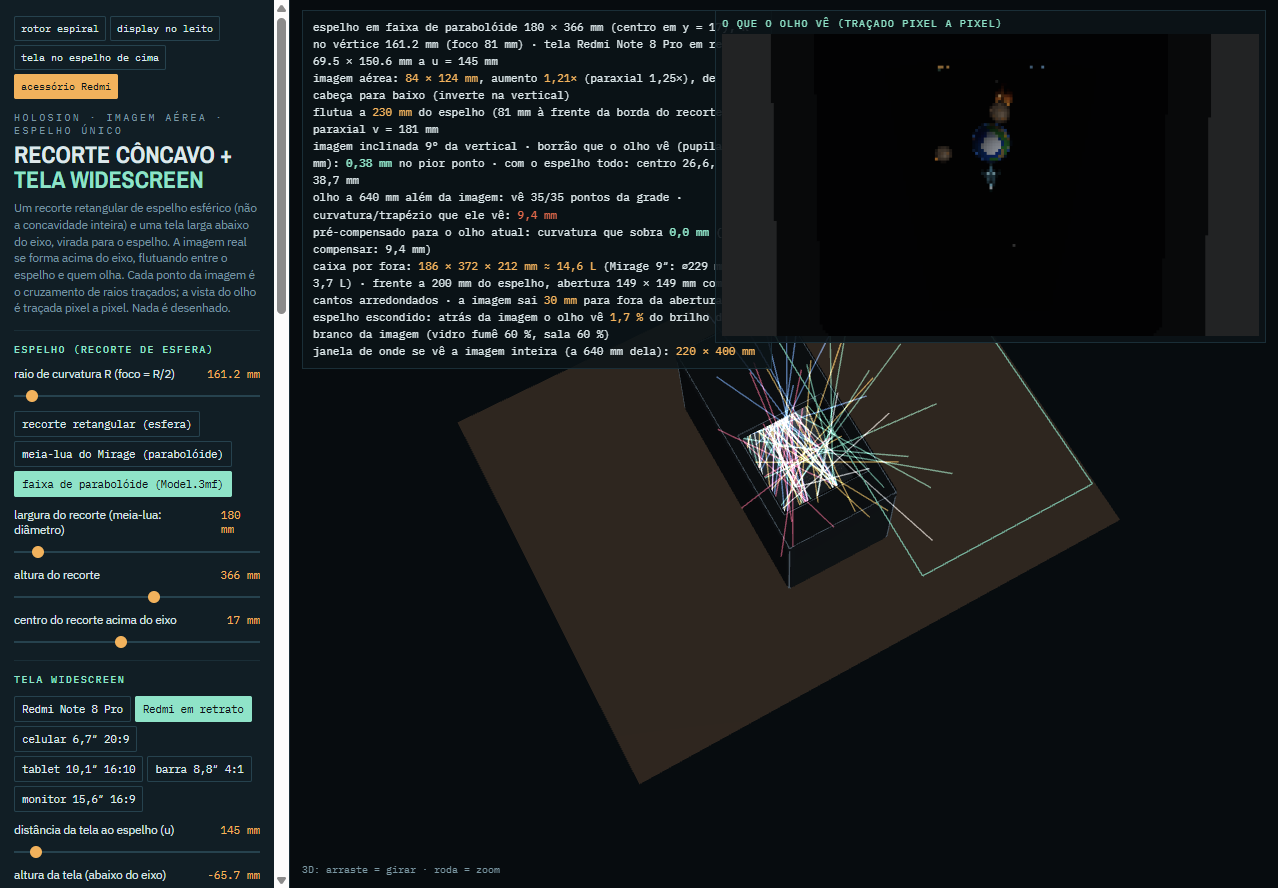
\includegraphics[width=\columnwidth]{jogo}
\caption{Jogo em tempo real no modo est\'ereo: Terra, nave e meteoro refeitos pelos dois olhos acima da abertura; a tela do telefone exibe as duas vistas pr\'e-distorcidas.}
\label{fig:jogo}
\end{figure}

\section{Discuss\~ao}
\paragraph{Tr\^es grandezas, um espelho} Uma tela plana em imagem real entrega a tela inteira e acomoda\c{c}\~ao correta, mas n\~ao pode entregar profundidade pr\'opria: os dois olhos amostram os mesmos pixels. Uma tela no plano focal entrega profundidade separando pixels por olho --- o princ\'ipio da fotografia integral~\cite{lippmann1908} aplicado a uma \'unica superf\'icie refletora --- mas s\'o v\^e a fra\c{c}\~ao da tela que cabe na abertura e paga o conflito verg\^encia--acomoda\c{c}\~ao. Resolver os tr\^es exigiria controle direcional por pixel (campo de luz)~\cite{wetzstein2012,lanman2013}, o que uma tela de telefone n\~ao oferece.

\paragraph{Quem governa o qu\^e} O teste de pixel isolou as duas fontes de erro: a precis\~ao de profundidade escala com o passo do pixel e com o quadrado da dist\^ancia do olho; o borr\~ao \'e independente da tela e vem da aberra\c{c}\~ao fora de foco do paraboloide~\cite{welford1986}. Por isso o iPhone melhora pouco e uma focal mais longa melhoraria mais.

\paragraph{Nitidez contra paralaxe} Alargar a abertura de 60 para 72~mm leva a excurs\~ao de $\pm$75 a $\pm$125~mm, mas o borr\~ao cresce com o quadrado do \^angulo fora de eixo (1,7 $\to$ 2,1~mm na borda) e os pixels compartilhados sobem a 3~\%. A inclina\c{c}\~ao do espelho n\~ao altera esse compromisso; apenas o gira para um \^angulo de observa\c{c}\~ao confort\'avel.

\paragraph{A arte que j\'a usa esta f\'isica} O que chamamos aqui de pr\'e-compensa\c{c}\~ao para o olho de projeto tem uma tradi\c{c}\~ao art\'istica longa: a anamorfose~\cite{baltrusaitis1977}. Felice Varini pinta formas geom\'etricas fragmentadas sobre pr\'edios e salas que s\'o se fecham num \'unico ponto de vista; Georges Rousse faz o mesmo com fotografia de interiores; Julian Beever e Edgar M\"uller desenham no ch\~ao figuras que ganham volume apenas da posi\c{c}\~ao da c\^amera. Em todos, a obra \'e a distor\c{c}\~ao calculada para um observador --- e desfaz-se com a paralaxe, exatamente como a tela pr\'e-distorcida da Se\c{c}\~ao~\ref{sec:recorte} desfaz-se quando o olho sai da janela. A fotografia integral de Lippmann~\cite{lippmann1908}, as impress\~oes lenticulares que dela descendem e as ilus\~oes de palco com vidro a 45$^\circ$ de Pepper~\cite{pepper1890} fazem o movimento inverso: usam a paralaxe a favor, dando a cada olho e a cada posi\c{c}\~ao uma vista pr\'opria. O acess\'orio est\'ereo deste trabalho pertence a essa segunda fam\'ilia, com a diferen\c{c}a de que a vista de cada olho \'e computada por tra\c{c}ado e n\~ao gravada.

\paragraph{Compara\c{c}\~ao com as p\'etalas} As p\'etalas da terceira aba atingem 0,20~mm porque disp\~oem de quatro telas, do espelho inteiro, de objeto menor e de olho mais pr\'oximo (360~mm), e porque nunca foram medidas com pupila finita. Sob a mesma r\'egua, o arranjo em cata-vento do acess\'orio borra 2,3~mm; \'e prov\'avel que a aba 3 compartilhe esse borr\~ao, o que fica como verifica\c{c}\~ao pendente.

\paragraph{O que n\~ao est\'a modelado} Emiss\~ao angular e contraste de OLED versus IPS, lat\^encia e erro do rastreio ocular (suposto perfeito), toler\^ancias de fabrica\c{c}\~ao do espelho, difra\c{c}\~ao nos pixels e espalhamento no vidro fum\^e. A sensibilidade de 0,03~mm ao foco indica que a altura do telefone precisa de ajuste fino na pe\c{c}a real.

\section{Conclus\~ao}
Um \'unico telefone e um \'unico recorte do espelho do Mirage produzem uma imagem a\'erea, mas o projetista tem de escolher: tela inteira sem conflito de foco (11,7~L, conte\'udo plano) ou profundidade real com uma pequena fra\c{c}\~ao da tela (4,4--5,2~L, conflito de 2--4~D). As geometrias finais foram exportadas em 3MF~\cite{mf3} com marcadores de olho e de volume para prototipagem, e um jogo interativo demonstra que cada configura\c{c}\~ao sustenta conte\'udo din\^amico em tempo real. A metodologia --- medir cada hip\'otese pelo mesmo tra\c{c}ado determin\'istico e registrar tamb\'em as refuta\c{c}\~oes --- foi o que impediu que ``configura\c{c}\~oes que pareciam funcionar'' sobrevivessem.

\section*{Disponibilidade}
Simuladores (HTML autocontidos sobre three.js~\cite{threejs}), especifica\c{c}\~ao, registro de medidas e arquivos 3MF acompanham o projeto~\cite{holosion2026}. Todos os n\'umeros deste texto s\~ao reproduz\'iveis a partir dos bot\~oes nomeados na quarta aba de \texttt{mirage-rotor-3d.html}.

\bibliographystyle{IEEEtran}
\bibliography{referencias}

\end{document}
